\documentclass{article}

\usepackage{graphicx}
\usepackage{amsmath}
\usepackage{fancyhdr}
\usepackage{float}
\usepackage[sorting=none]{biblatex}
\usepackage[margin=1in]{geometry}
\usepackage[font={small,it}]{caption}
\usepackage{placeins}
\usepackage{xepersian}

%\DeclareMathOperator*{\btie}{\bowtie}
\addbibresource{bibliography.bib}
\settextfont[Scale=1.2]{B-NAZANIN.TTF}
\setlatintextfont[Scale=1]{Times New Roman}
\renewcommand{\baselinestretch}{1.5}
\pagestyle{fancy}
\fancyhf{}
\rhead{تکلیف اول آزمایشگاه شبکه ‌های کامپیوتری}
\lhead{\thepage}
\rfoot{علیرضا ابره فروش}
\lfoot{9816603}
\renewcommand{\headrulewidth}{1pt}
\renewcommand{\footrulewidth}{1pt}

\begin{document}
\begin{titlepage}
\begin{center}

\includegraphics[width=0.4\textwidth]{figures/IUT Logo.png}\\
        
\LARGE
\textbf{دانشگاه صنعتی اصفهان}\\
\textbf{دانشکده مهندسی برق و کامپیوتر}\\
        
\vfill
        
\huge
\textbf{عنوان: تکلیف چهارم درس ریزپردازنده}\\
        
\vfill
        
\LARGE
\textbf{نام و نام خانوادگی: علیرضا ابره فروش}\\
\textbf{شماره دانشجویی: 9816603}\\
\textbf{نیم\,سال تحصیلی: پاییز 1400}\\
\textbf{مدرّس: دکتر عارف کریمی افشار}\\
\end{center}
\end{titlepage}


%\tableofcontents
\newpage



\section{گام اول}
ابتدا به مسیر
\lr{Start/Control panel/Network and Internet/Network and Sharing center/}
می‌رویم.
\begin{figure}[H]
    \centering
    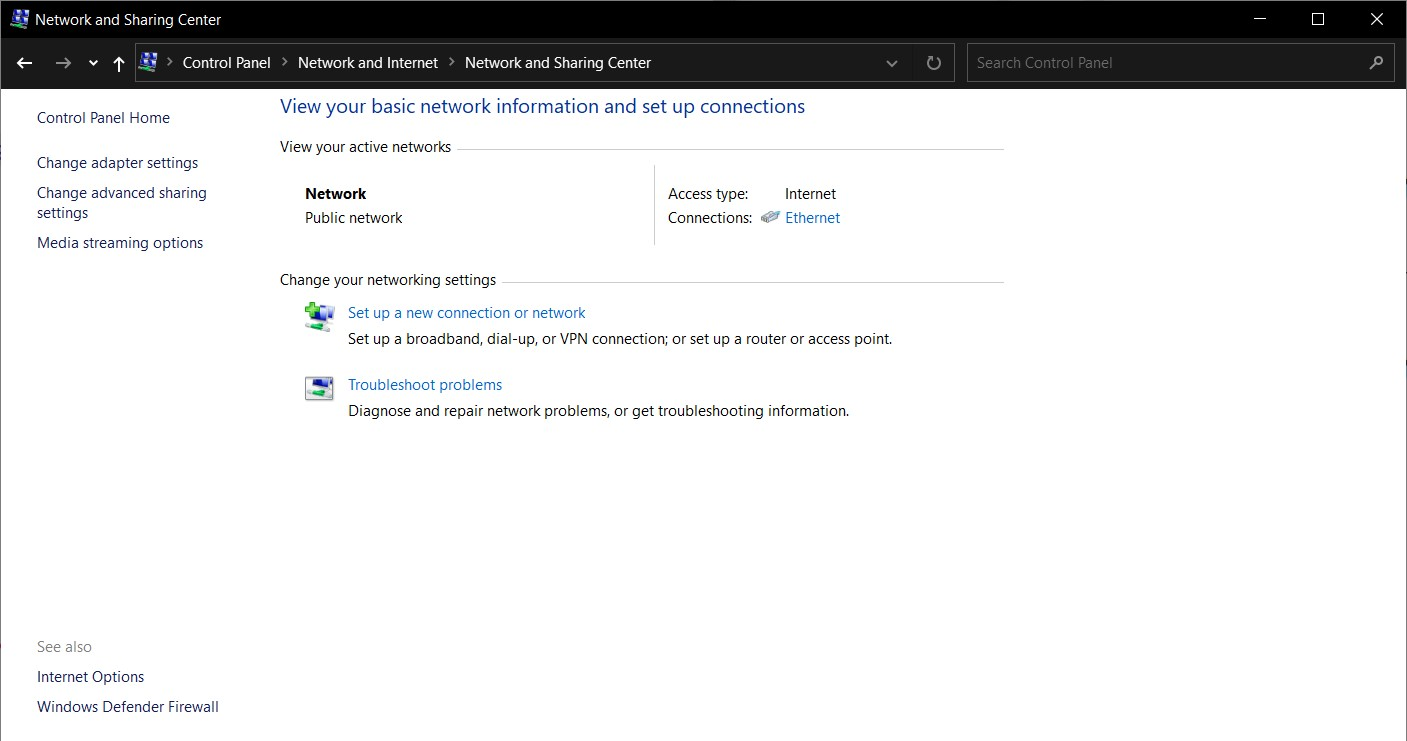
\includegraphics[width=1.0\textwidth]{figures/1.1.jpg}
    \caption
	{
\lr{Start/Control panel/Network and Internet/Network and Sharing center/}
	}
    \label{fig:fig1}
\end{figure}
سپس روی \lr{Ethernet} که شبکه فعال هست کلیک می‌کنیم.
\begin{figure}[H]
    \centering
    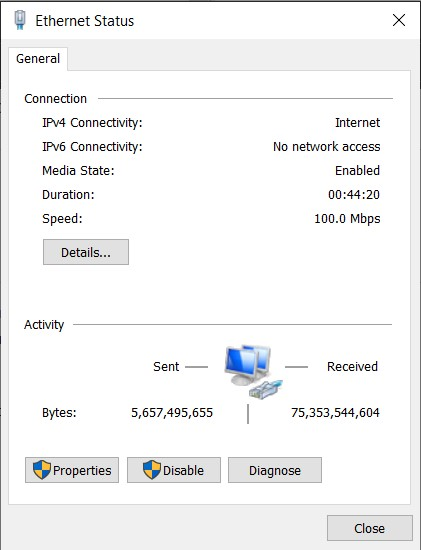
\includegraphics[width=0.3\textwidth]{figures/1.2.jpg}
    \caption
	{
\lr{Ethernet Status}
	}
    \label{fig:fig1}
\end{figure}
حال روی دکمه‌ی \lr{Details} کلیک می‌کنیم.
\begin{figure}[H]
    \centering
    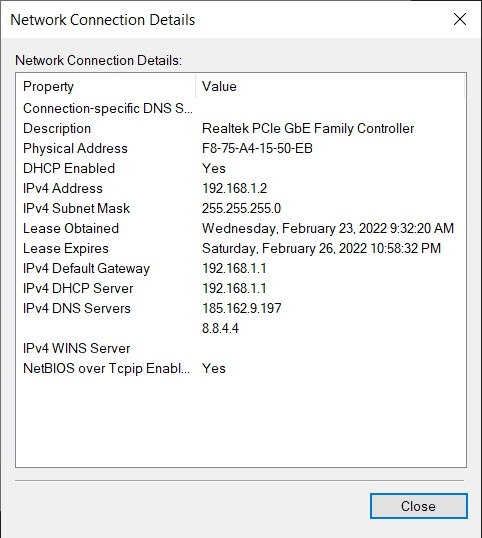
\includegraphics[width=0.5\textwidth]{figures/1.3.jpg}
    \caption
	{
\lr{Network Connection Details}
	}
    \label{fig:fig1}
\end{figure}
با مشاهده پنجره‌ی بالا درمی‌یابیم که آدرس سیستم(\lr{IPv4}) و \lr{Gateway} به ترتیب برابر 2.1.168.192 و 1.1.168.192 است. با توجه به اینکه بایت بالای آن‌ها 192 است از \lr{Class C} هستند. همچنین موارد مذکور را می‌توان از طریق محیط \lr{Command Prompt} و با وارد کردن دستور \lr{ipconfig} به دست آورد.

\section{گام دوم}
 ابتدا مطابق فیلم آموزشی جلسه اول پوشه‌ی \lr{test} را می‌سازیم و با راست کلیک روی آن وارد \lr{Properties} می‌شویم.
\begin{figure}[H]
    \centering
    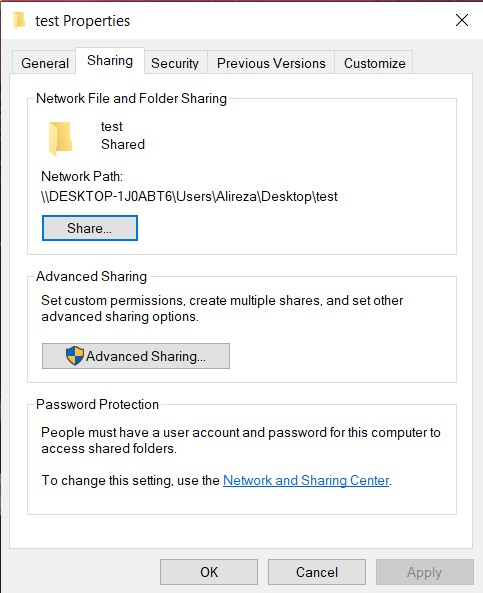
\includegraphics[width=0.5\textwidth]{figures/2.1.jpg}
    \caption
	{
\lr{test Properties}
	}
    \label{fig:fig1}
\end{figure}
حال در تب \lr{Sharing} بر روی \lr{Share} کلیک می‎‌کنیم.
\begin{figure}[H]
    \centering
    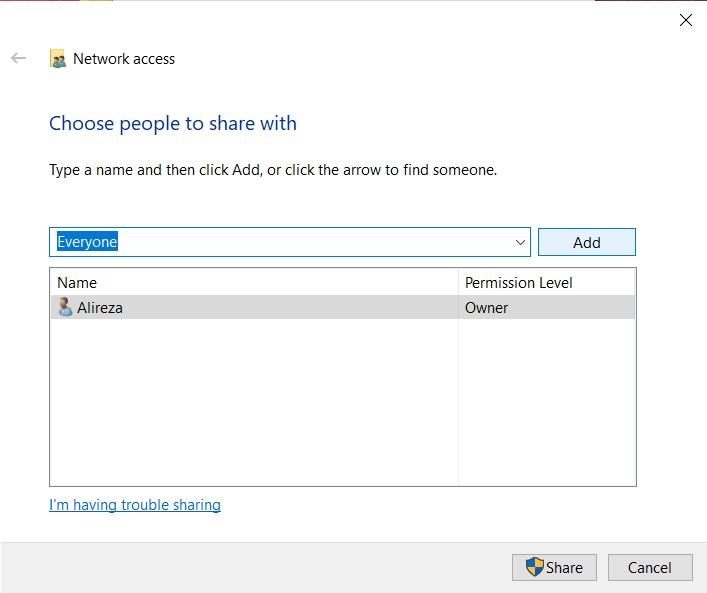
\includegraphics[width=0.5\textwidth]{figures/2.2.jpg}
    \caption
	{
\lr{Network access}
	}
    \label{fig:fig1}
\end{figure}
حال دسترسی به پوشه را با انتخاب و اضافه کردن گزینه \lr{Everyone} به همه‌ی کاربران می‌دهیم.
\begin{figure}[H]
    \centering
    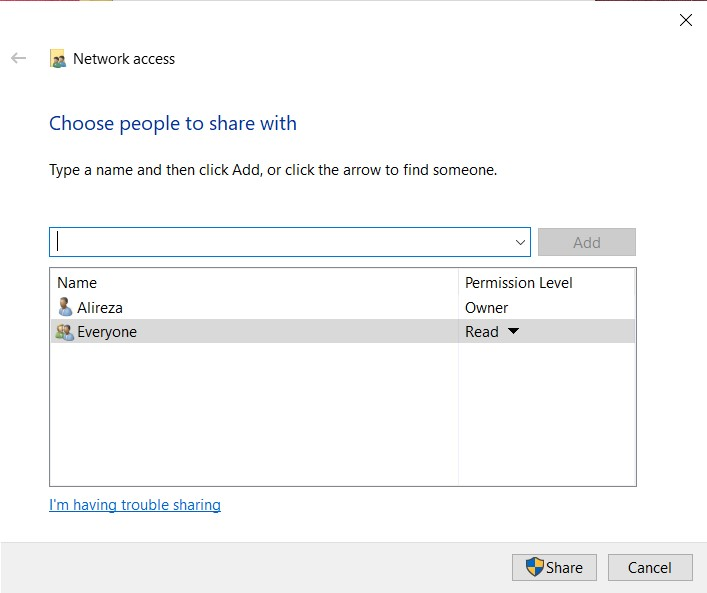
\includegraphics[width=0.5\textwidth]{figures/2.3.jpg}
    \caption
	{
\lr{Network access}
	}
    \label{fig:fig1}
\end{figure}
سطح دسترسی خواندن و نوشتن را برای این پوشه به \lr{Everyone} می‌دهیم.
\begin{figure}[H]
    \centering
    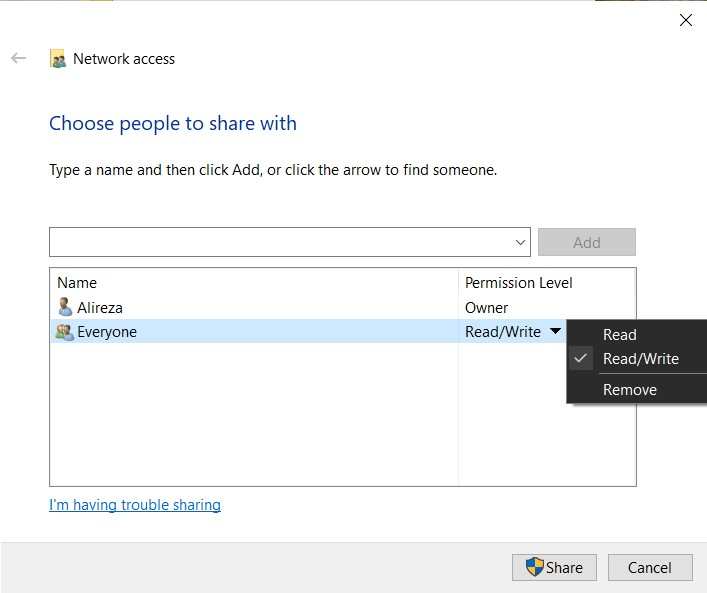
\includegraphics[width=0.5\textwidth]{figures/2.4.jpg}
    \caption
	{
\lr{Network access}
	}
    \label{fig:fig1}
\end{figure}
مجدد به تب \lr{Sharing} می‌رویم و روی \lr{Advanced Sharing} کلیک می‌کنیم. برای به اشتراک گذاشتن پوشه حتما باید تیک \lr{Share this folder} را بزنیم.
\begin{figure}[H]
    \centering
    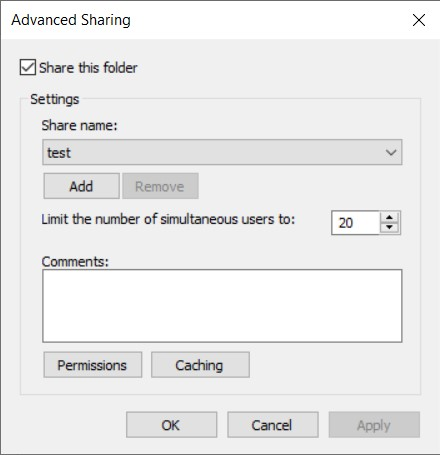
\includegraphics[width=0.5\textwidth]{figures/2.5.jpg}
    \caption
	{
\lr{Advanced Sharing}
	}
    \label{fig:fig1}
\end{figure}
برای بررسی اینکه پوشه به اشتراک گذاشته شده است از طریق \lr{Run} و وارد کردن آدرس سیستم به شکل زیر اقدام می‌کنیم.

\begin{figure}[H]
    \centering
    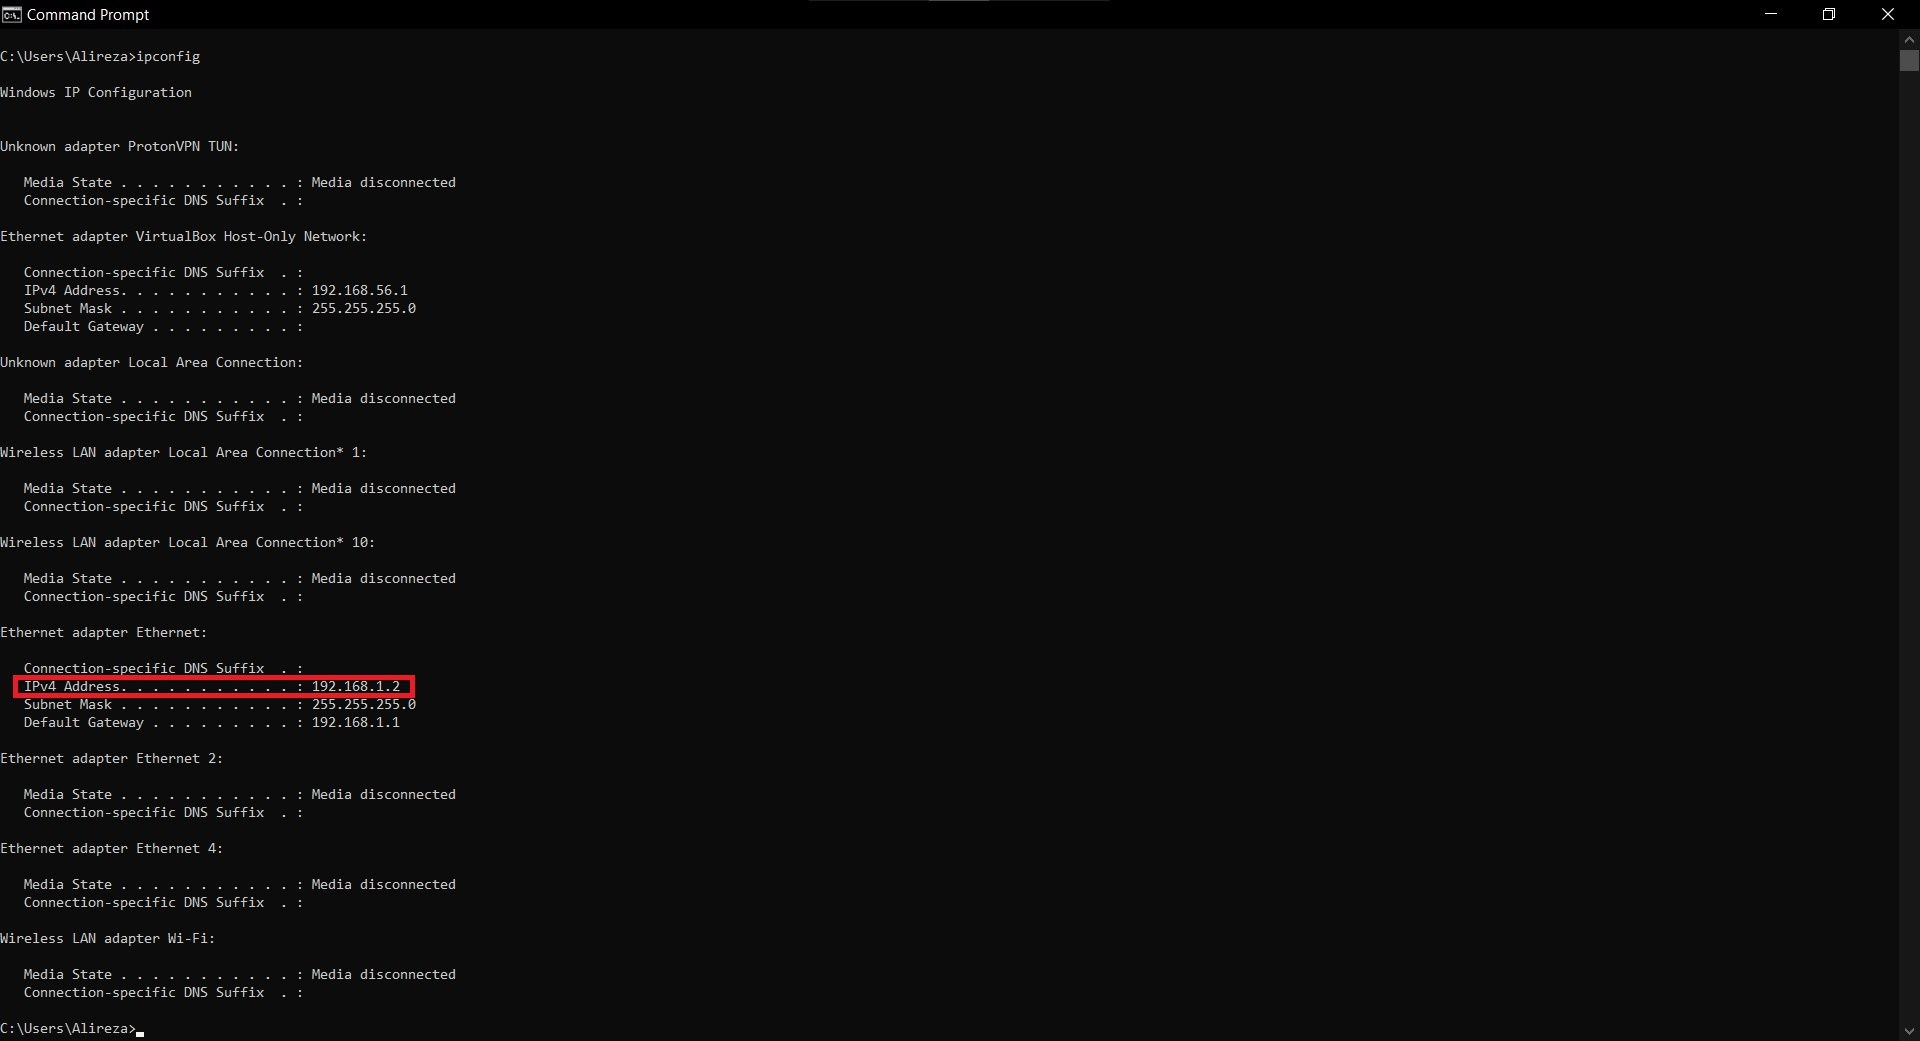
\includegraphics[width=1.0\textwidth]{figures/2.6.jpg}
    \caption
	{
\lr{finding my address}
	}
    \label{fig:fig1}
\end{figure}

\begin{figure}[H]
    \centering
    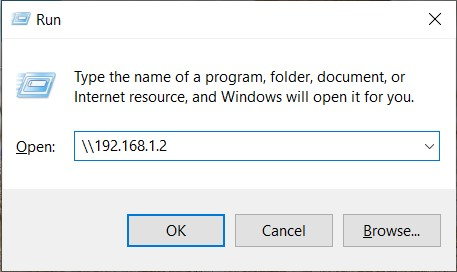
\includegraphics[width=0.5\textwidth]{figures/2.7.jpg}
    \caption
	{
\lr{Run}
	}
    \label{fig:fig1}
\end{figure}

\begin{figure}[H]
    \centering
    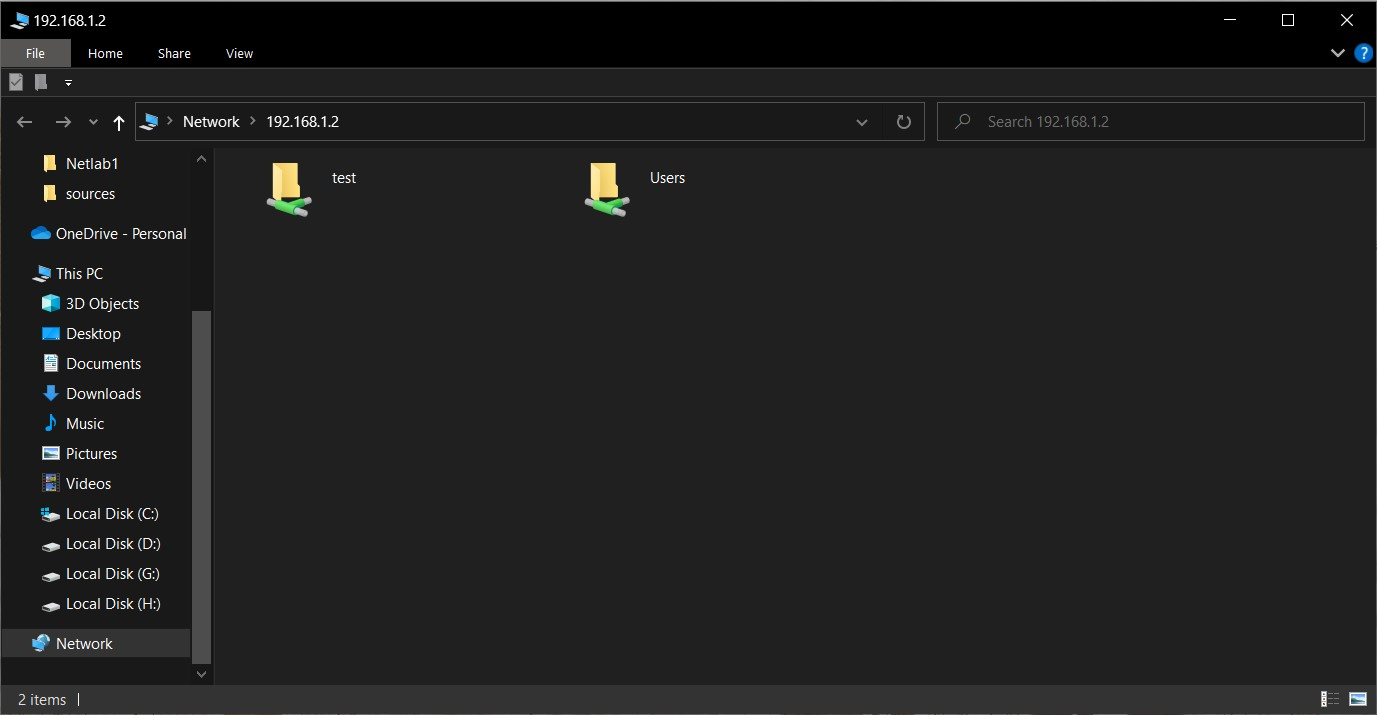
\includegraphics[width=1.0\textwidth]{figures/2.8.jpg}
    \caption
	{
پوشه‌ها
	}
    \label{fig:fig1}
\end{figure}
می‌بینیم که پوشه‌ی \lr{test} به اشتراک گذاشته شده است.

\section{گام سوم}
\begin{figure}[H]
    \centering
    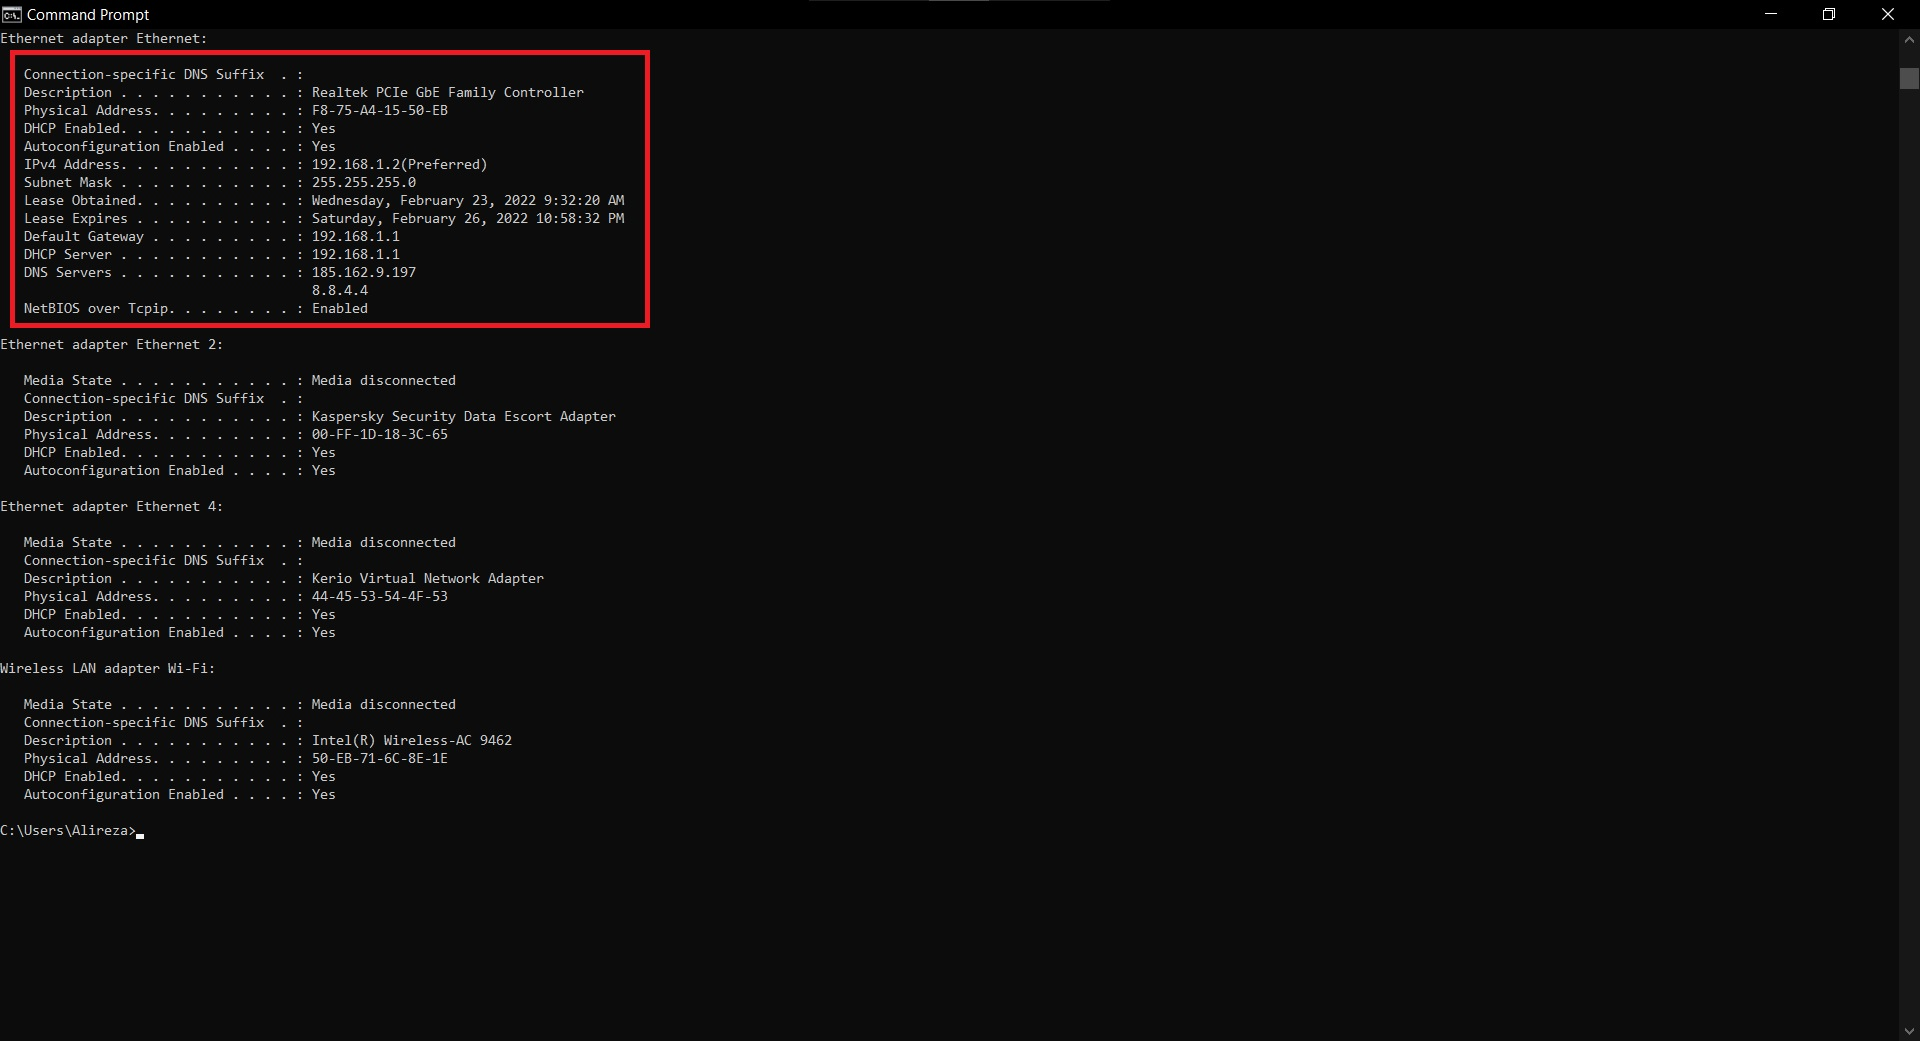
\includegraphics[width=1.0\textwidth]{figures/3.1.jpg}
    \caption
	{
بخشی از خروجی دستور \lr{ipconfig /all}
	}
    \label{fig:fig1}
\end{figure}

\subsection{}
آدرس فیزیکی(\lr{Mac Address}) \lr{F8-75-A4-15-50-EB} است.
\subsection{}
آدرس سرور نام(\lr{DNS Servers}) \lr{185.162.9.197
                                       8.8.4.4} است.
\subsection{}
دستور \lr{ipconfig /all} جزئیات بیشتری از کانفیگریشن شبکه نسبت به حالت بدون \lr{/all} را می‌دهد.
\subsection{}
\lr{DHCP Enabled} نشانگر آن است که آیا \lr{DHCP Server} آدرس سیستم را به صورت اتوماتیک تنظیم کرده است یا خیر. از آنجایی که در خروجی بالا \lr{Yes} است پس آدرس سیستم به صورت اتوماتیک تنظیم شده است. برای تنظیم دستی آن می‌توان به شکل زیر عمل کرد:\\
ابتدا وارد \lr{Network and Sharing Center} در کنترل پنل می‌شویم و روی \lr{Change adapter settings} کلیک می‌کنیم.
\begin{figure}[H]
    \centering
    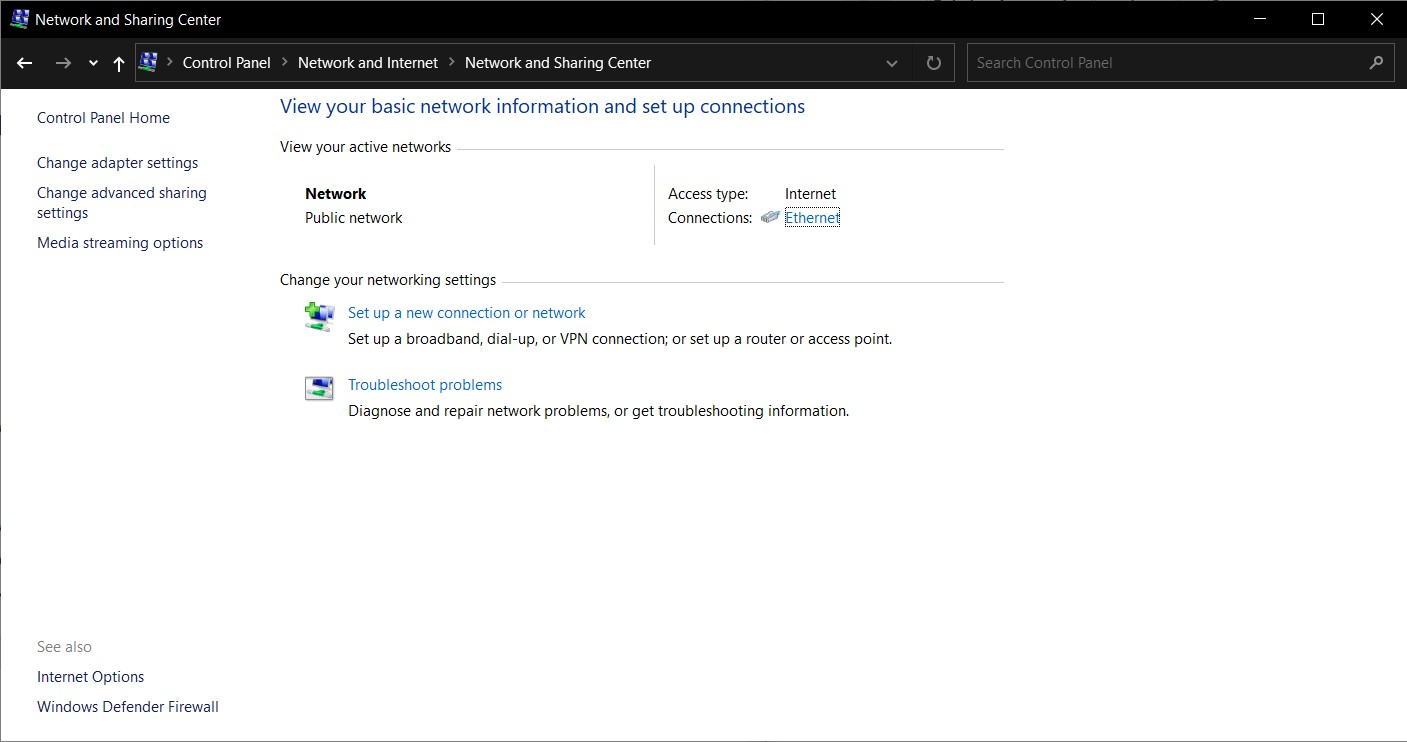
\includegraphics[width=1.0\textwidth]{figures/3.4.1.jpg}
    \caption
	{
\lr{Control Panel/Network and Internet/Network and Sharing Center}
	}
    \label{fig:fig1}
\end{figure}
حال بر روی شبکه مورد نظر راست کلیک می‌کنیم و وارد \lr{Properites} آن می‌شویم.
\begin{figure}[H]
    \centering
    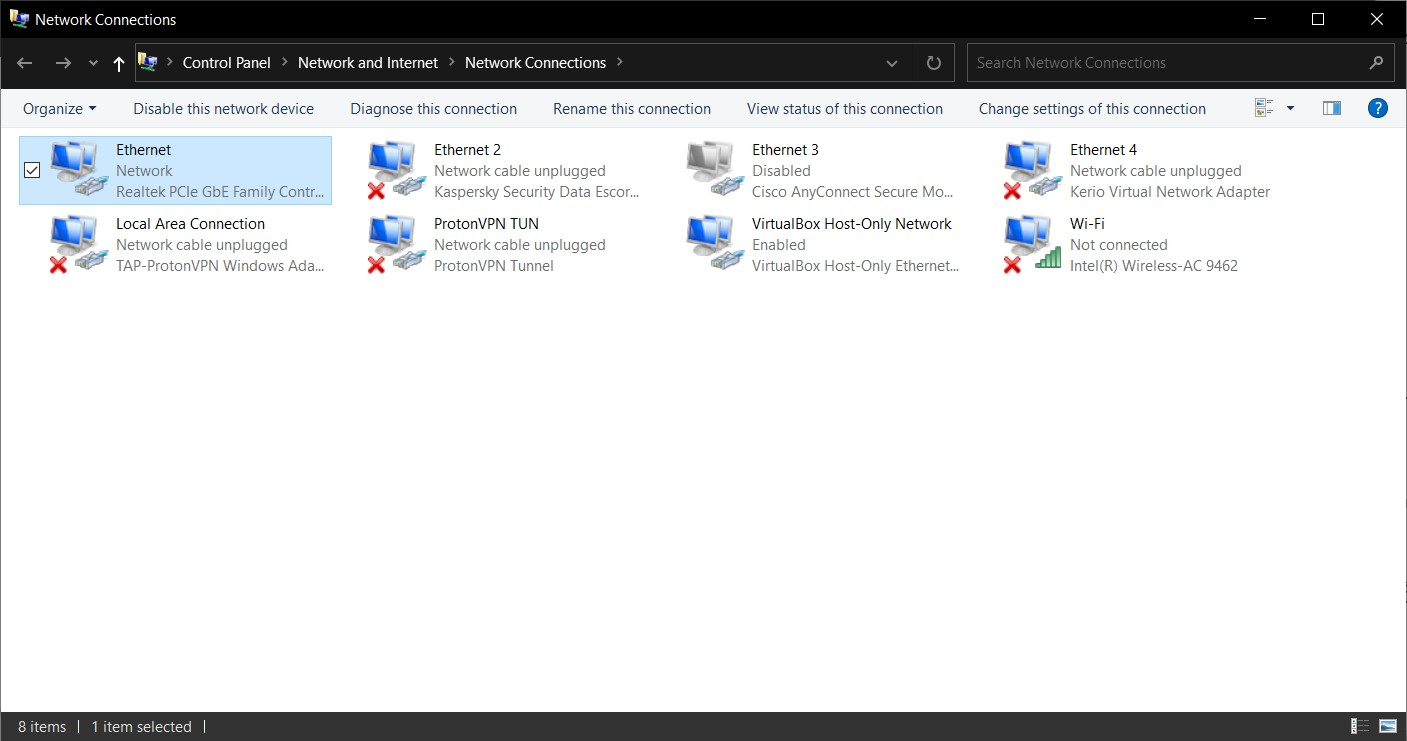
\includegraphics[width=1.0\textwidth]{figures/3.4.2.jpg}
    \caption
	{
\lr{Control Panel/Network and Internet/Network Connections}
	}
    \label{fig:fig1}
\end{figure}
مورد \lr{Internet Protocol Version 4 (TCP/IPv4)} را انتخاب و سپس روی \lr{Properties} کلیک می‌کنیم.
\begin{figure}[H]
    \centering
    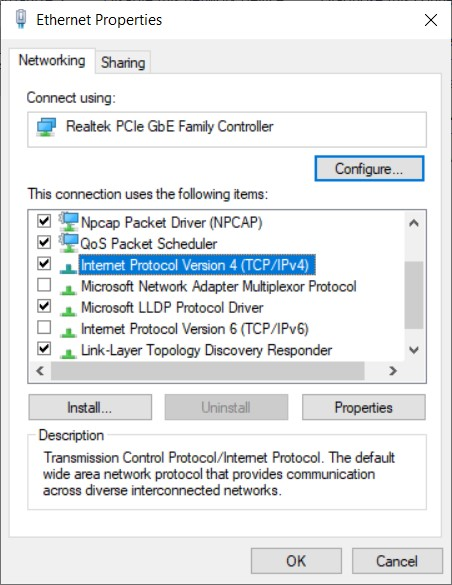
\includegraphics[width=0.5\textwidth]{figures/3.4.3.jpg}
    \caption
	{
\lr{Ethernet Properties}
	}
    \label{fig:fig1}
\end{figure}
با انتخاب \lr{Use the following IP address} می‌توان به صورت دستی آدرس سیستم را تنظیم کرد.
\begin{figure}[H]
    \centering
    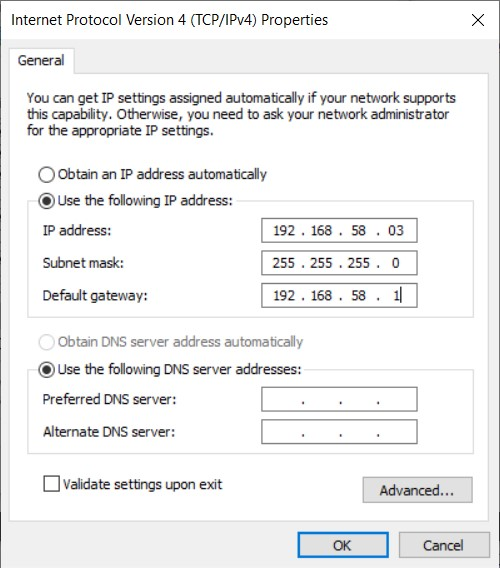
\includegraphics[width=0.3\textwidth]{figures/3.4.4.jpg}
    \caption
	{
\lr{Internet Protocol Version 4 (TCP/IPv4) Properties}
	}
    \label{fig:fig1}
\end{figure}


\subsection{}
\lr{release} کارت شبکه را غیرفعال می‌کند. در واقع کلاینت را فورس می‌کند که با فرستادن یک \lr{DHCP release notification} آدرس \lr{IP} فعلی را آزاد کند.
\begin{figure}[H]
    \centering
    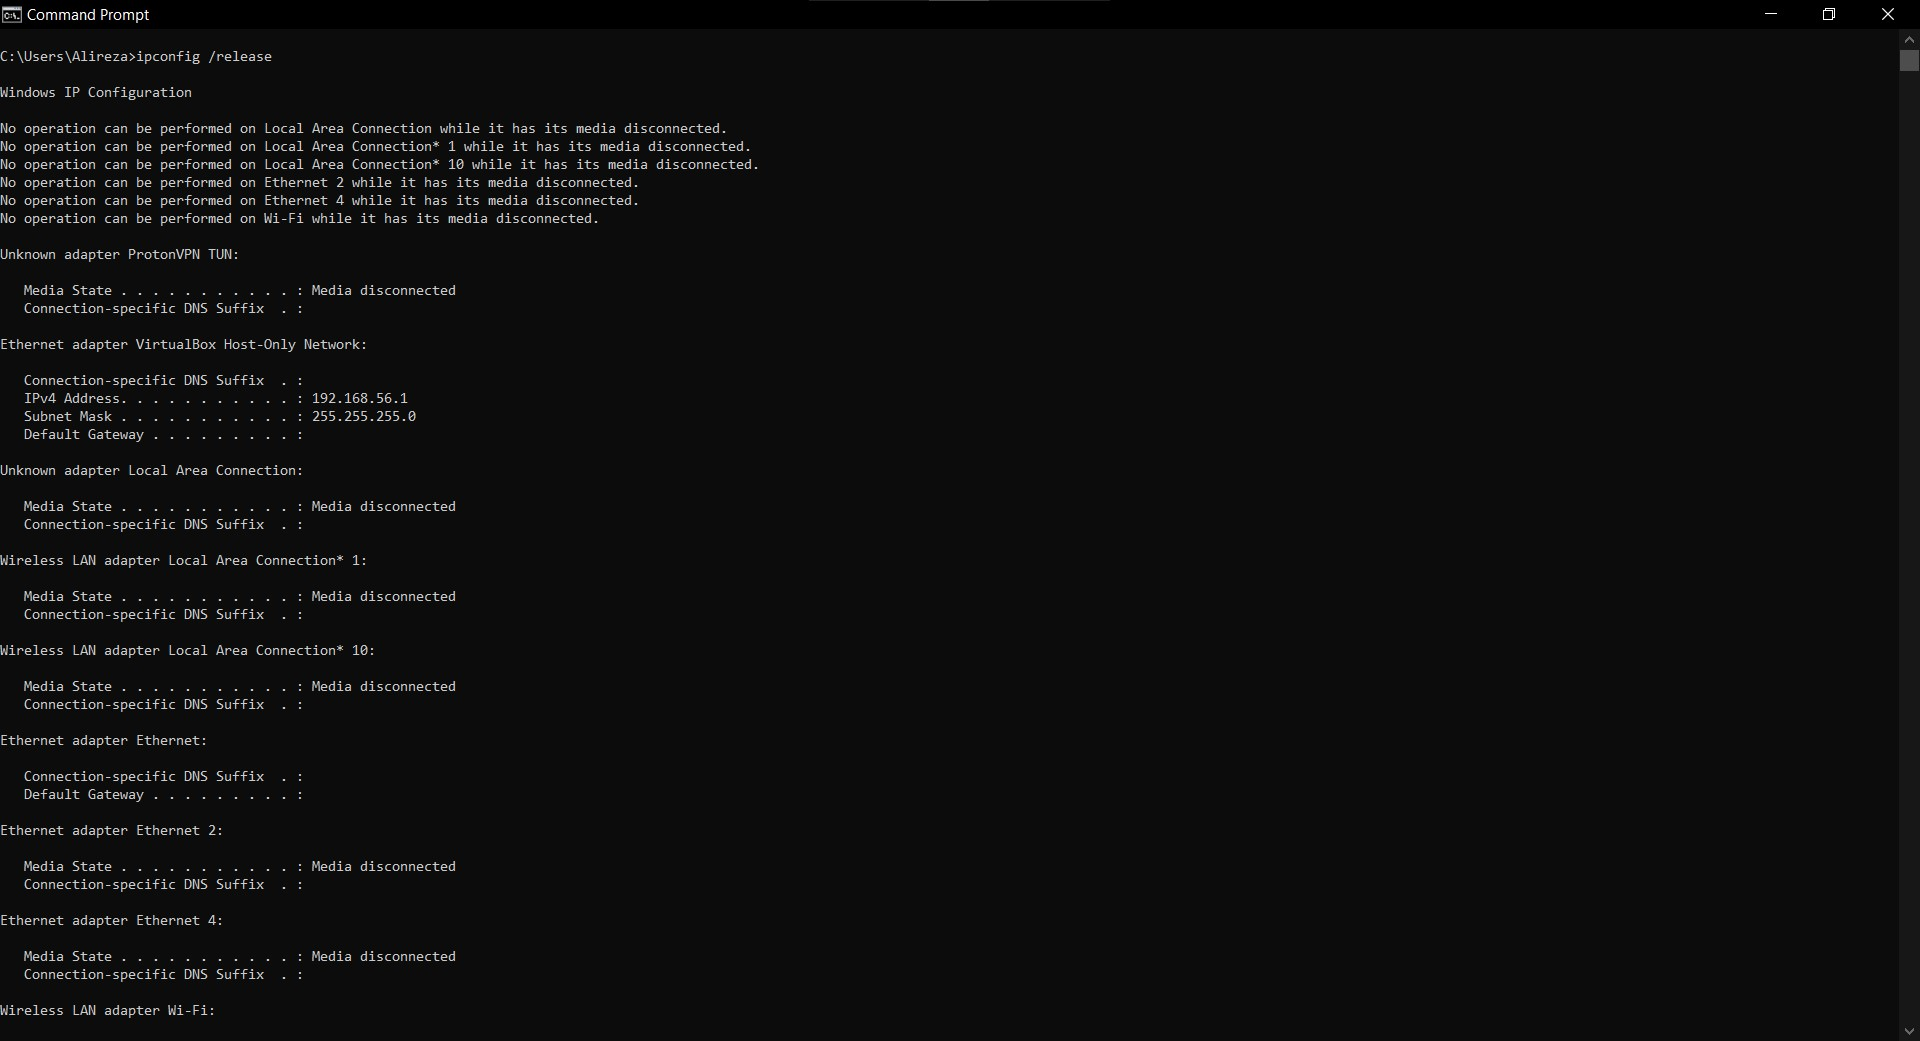
\includegraphics[width=1.0\textwidth]{figures/3.5.1.jpg}
    \caption
	{
\lr{ipconfig /release}
	}
    \label{fig:fig1}
\end{figure}

\begin{figure}[H]
    \centering
    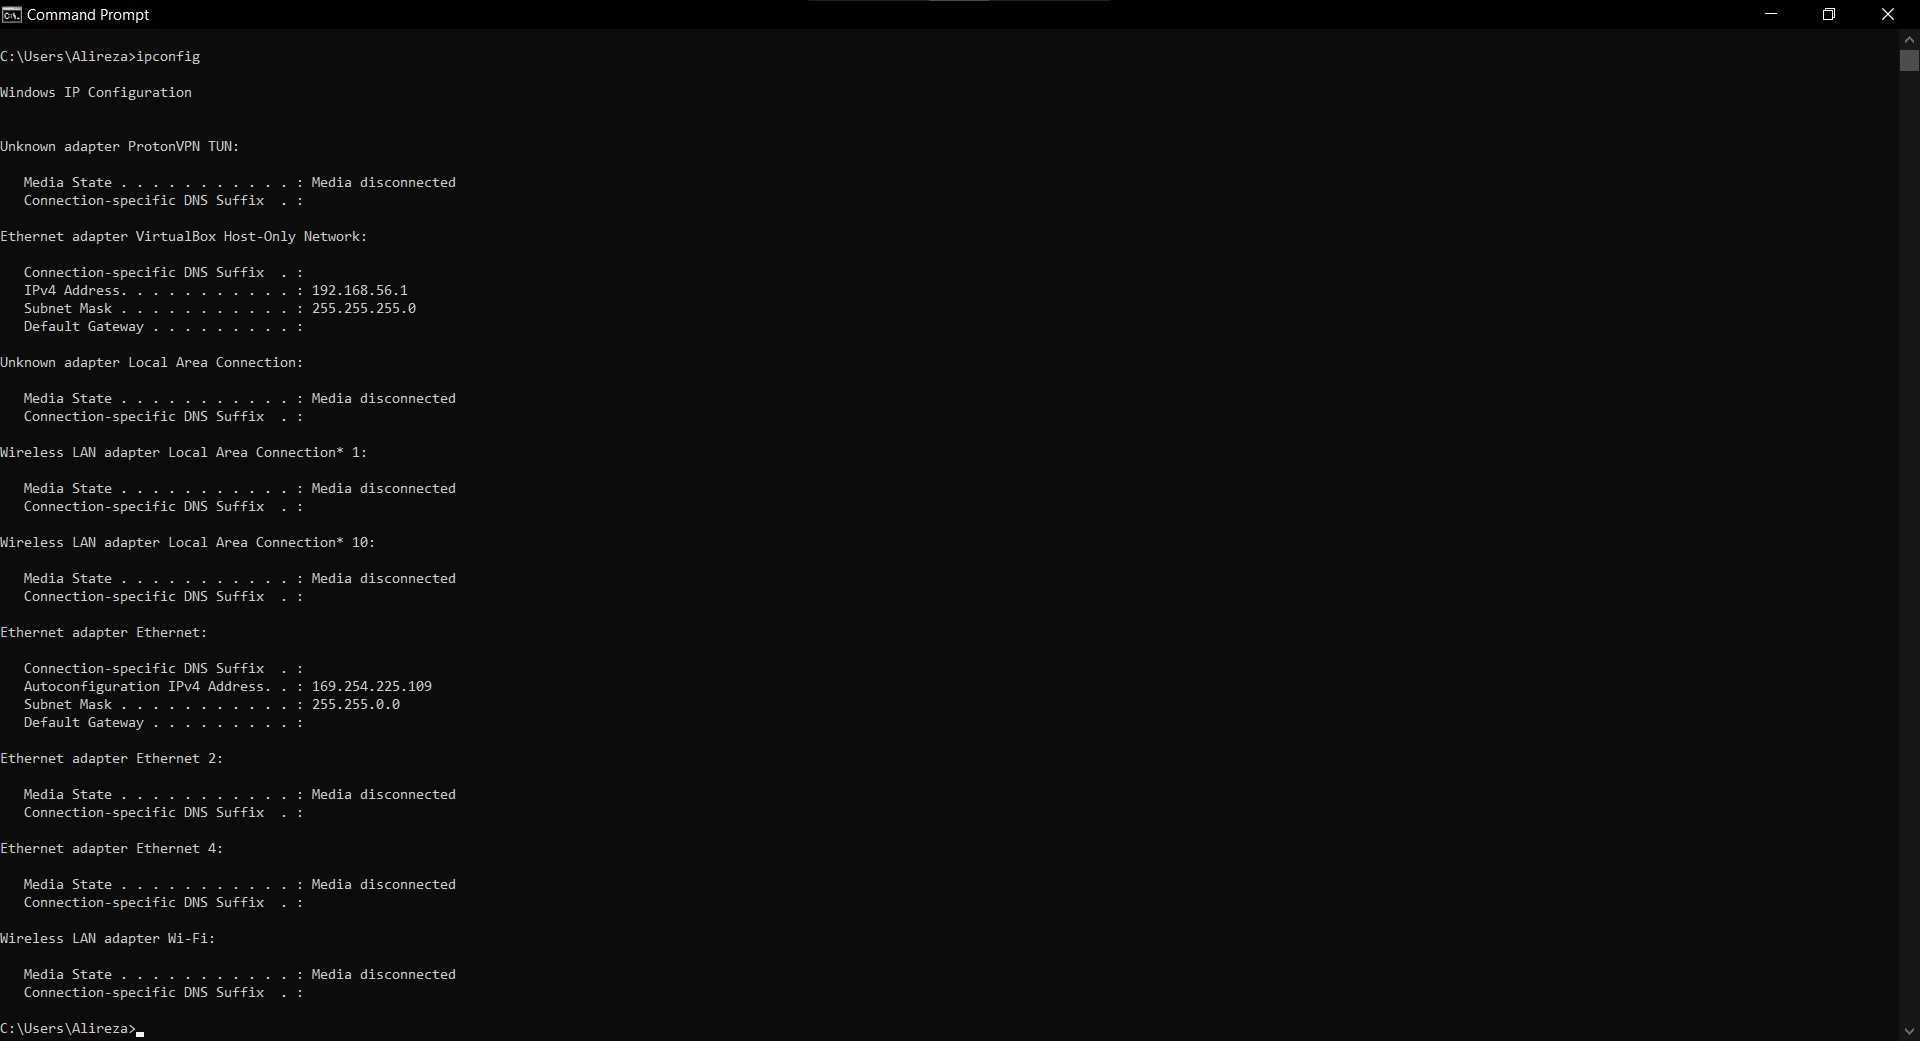
\includegraphics[width=1.0\textwidth]{figures/3.5.2.jpg}
    \caption
	{
\lr{ipconfig}
	}
    \label{fig:fig1}
\end{figure}

\subsection{}
\lr{renew} کارت شبکه را فعال می‌کند. در واقع کلاینت را فورس می‌کند که از \lr{DHCP server} یک آدرس \lr{IP} بر روی روتر بگیرد.
\begin{figure}[H]
    \centering
    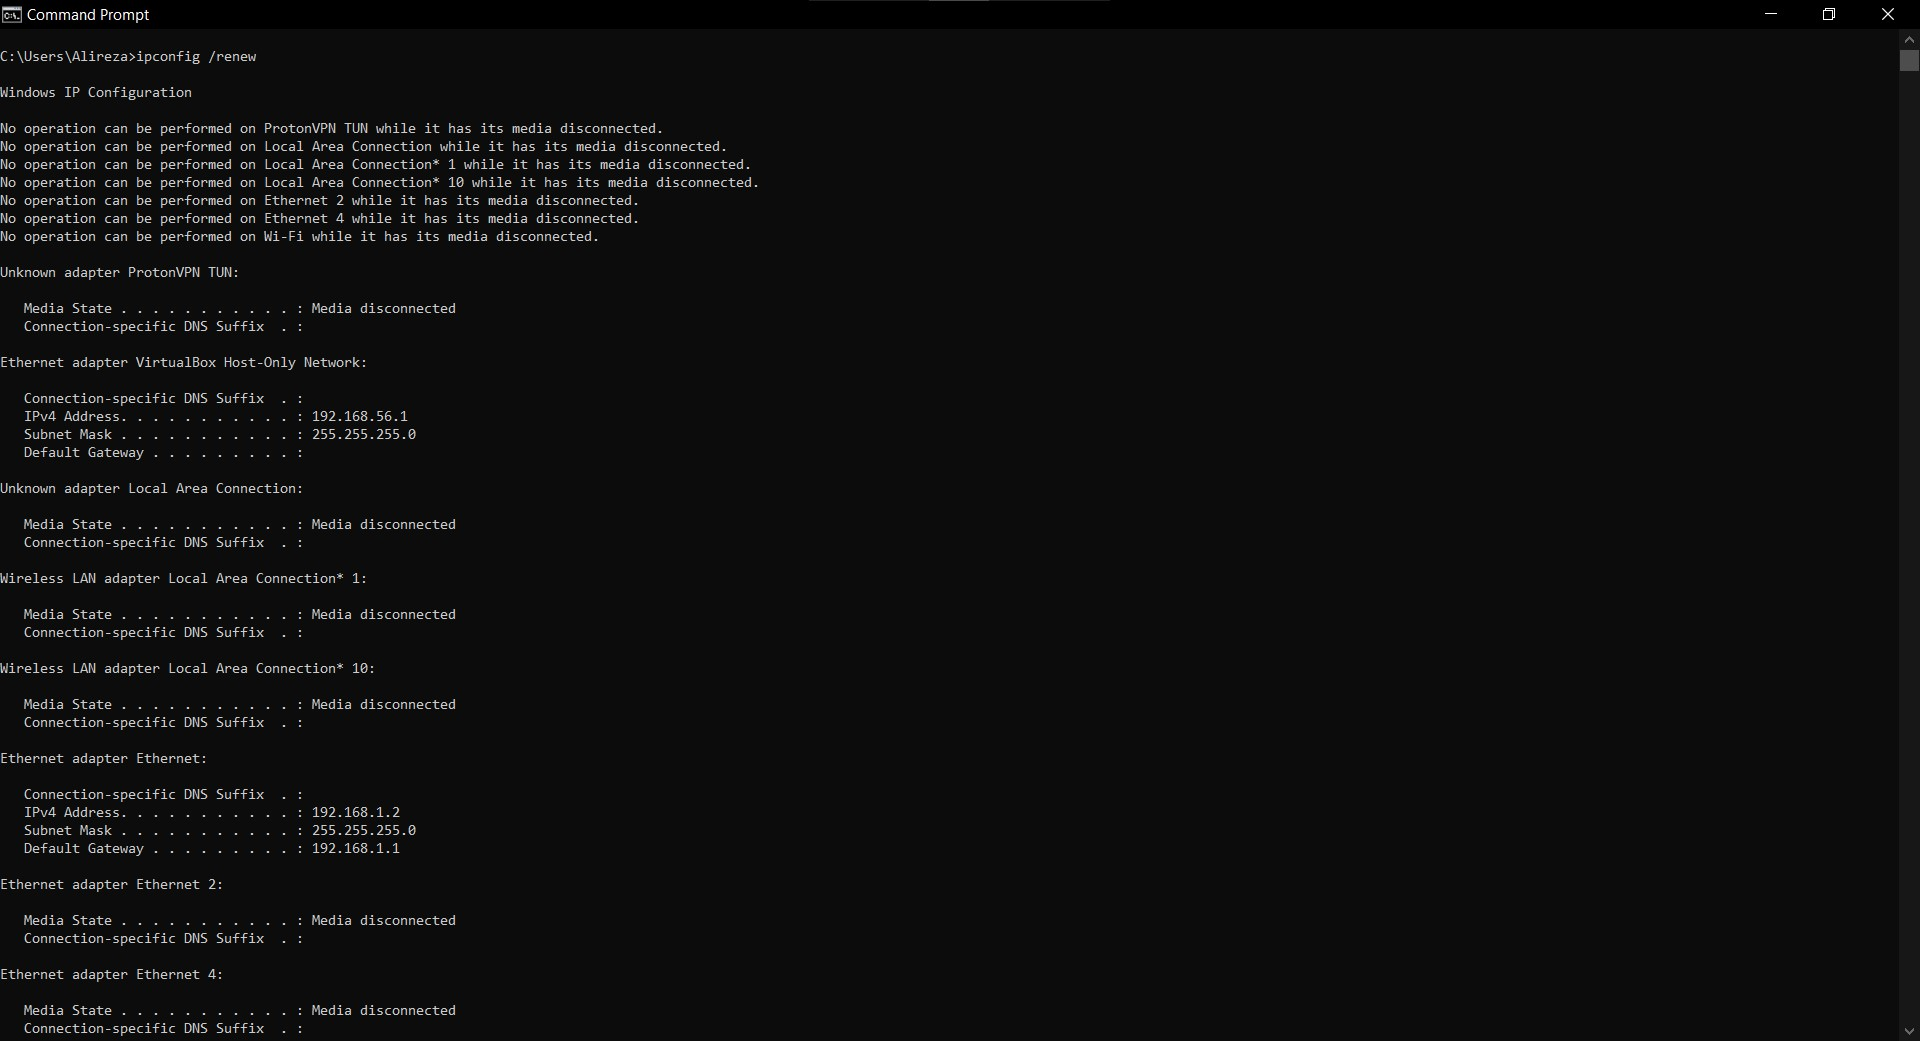
\includegraphics[width=1.0\textwidth]{figures/3.6.1.jpg}
    \caption
	{
\lr{ipconfig /renew}
	}
    \label{fig:fig1}
\end{figure}

\begin{figure}[H]
    \centering
    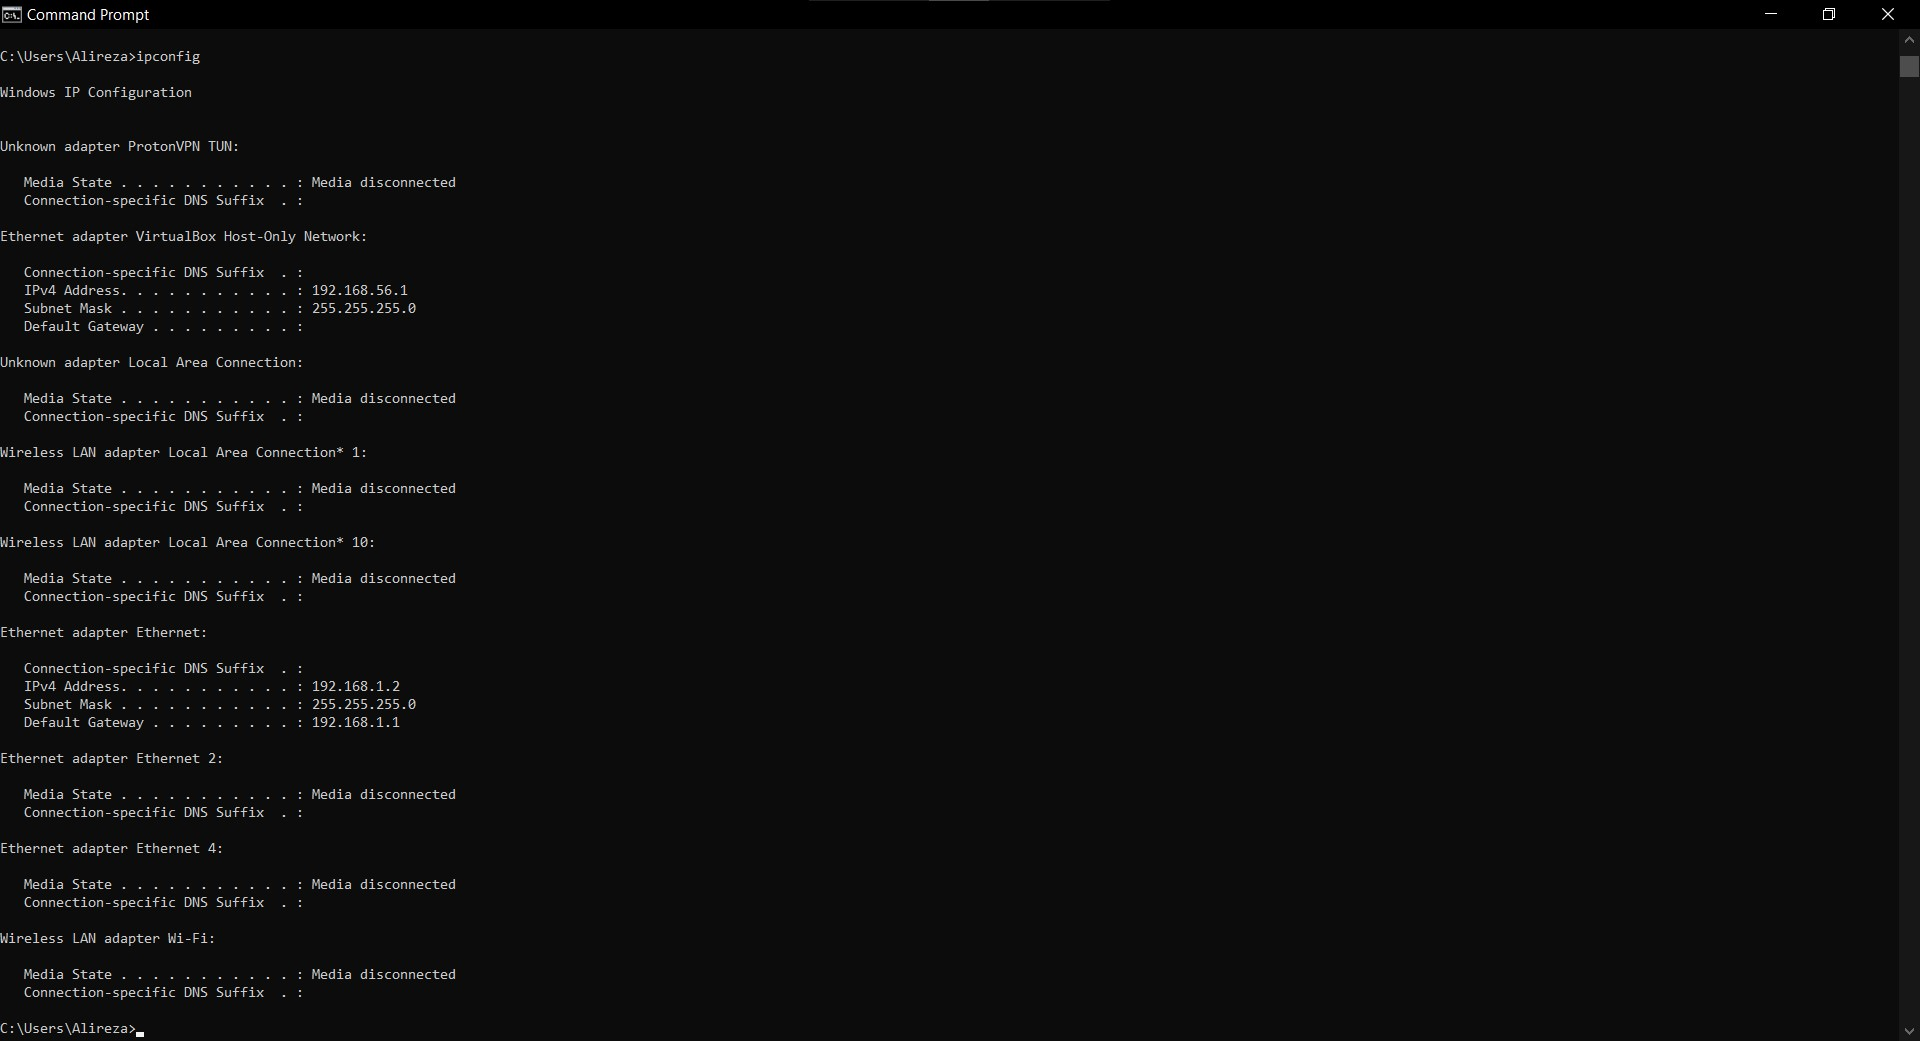
\includegraphics[width=1.0\textwidth]{figures/3.6.2.jpg}
    \caption
	{
\lr{ipconfig}
	}
    \label{fig:fig1}
\end{figure}

\subsection{}
\lr{getmac} به طور خاص آدرس فیزیکی را برمی‌گرداند.

\section{گام چهارم}
\begin{figure}[H]
    \centering
    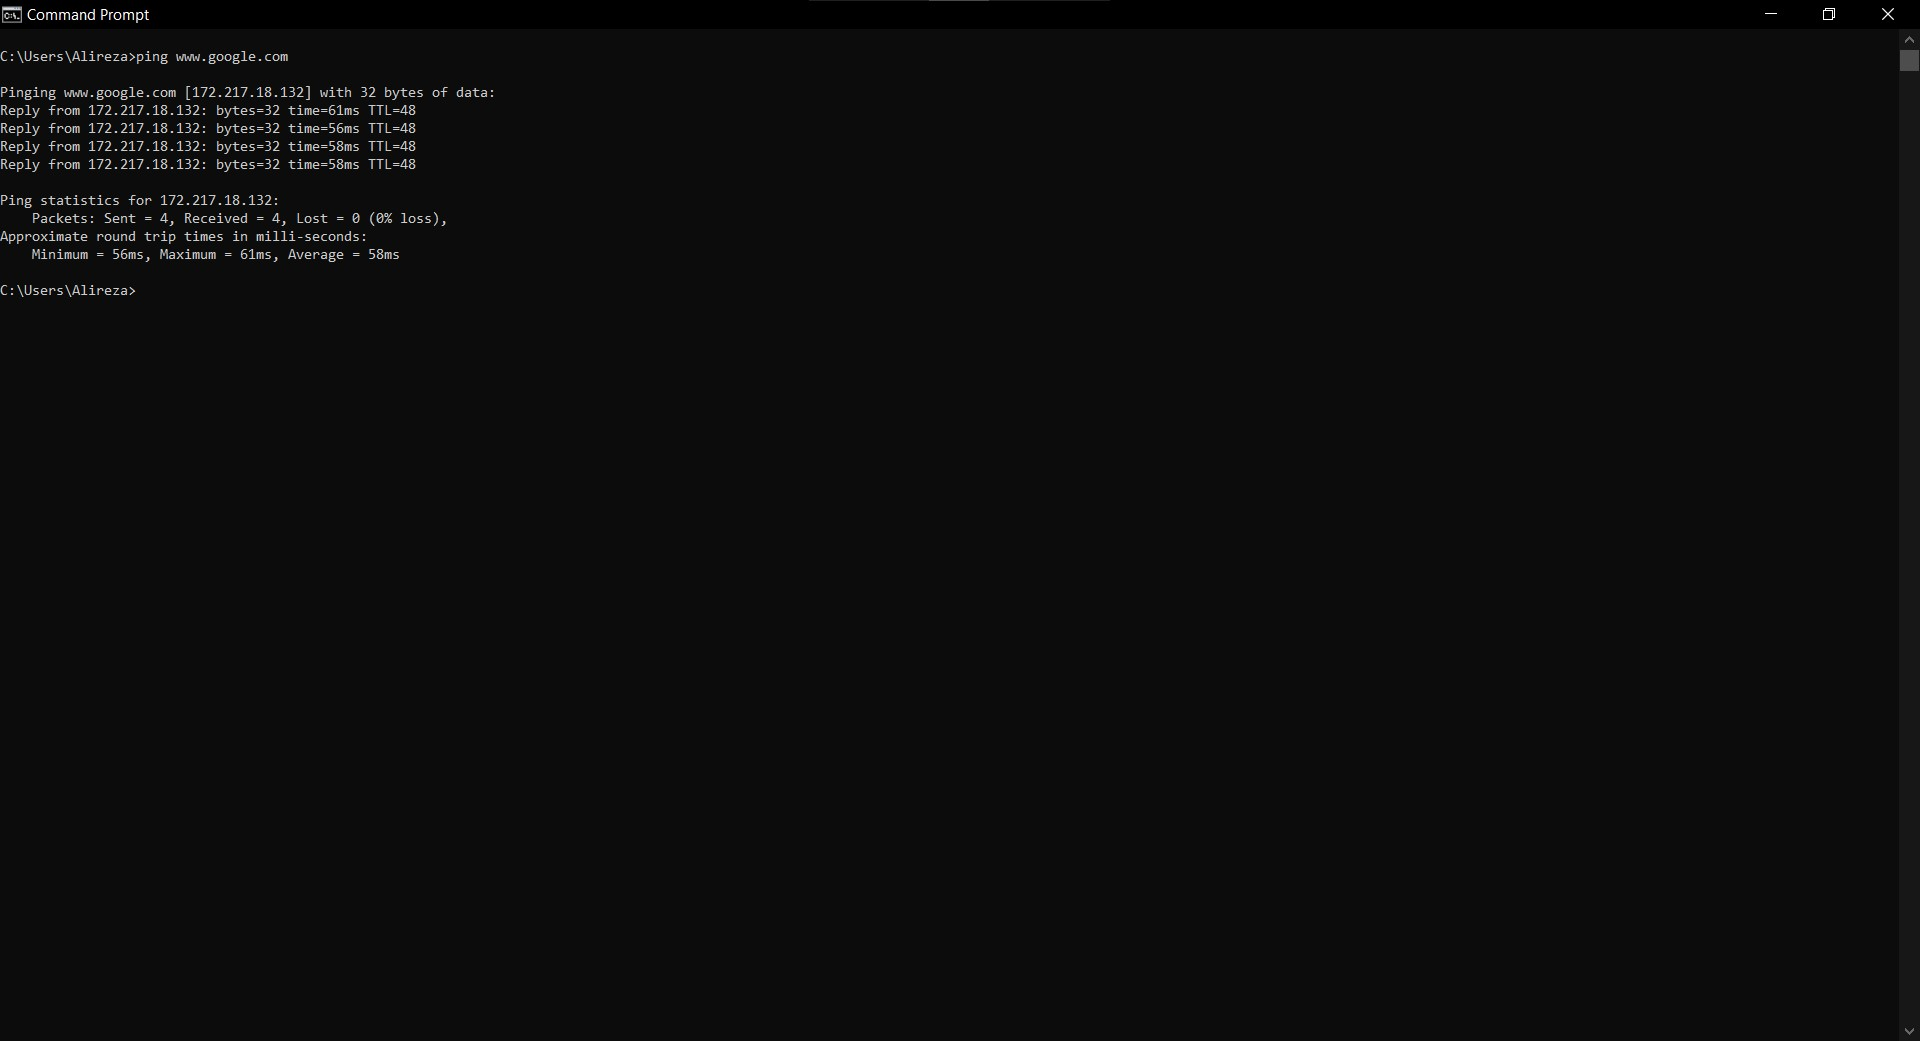
\includegraphics[width=1.0\textwidth]{figures/4.1.jpg}
    \caption
	{
\lr{ping www.google.com}
	}
    \label{fig:fig1}
\end{figure}
چون \lr{Reply} دریافت کردیم پس ارتباطمان با \lr{www.google.com} برقرار است.

\section{گام پنجم}
دستور \lr{tracert} به ما نشان می‌دهد که چه روترهایی با چه آدرس‌هایی در مسیر رسیدن بسته‌ی ما تا \lr{target} مورد نظر وجود دارد. اولین آدرسی که مشاهده می‌کنیم \lr{Default gateway} است. ماکسیمم 30 هم بیانگر این است که حداکثر تا 30 هاپ را می‌توان \lr{trace} کرد.
\begin{figure}[H]
    \centering
    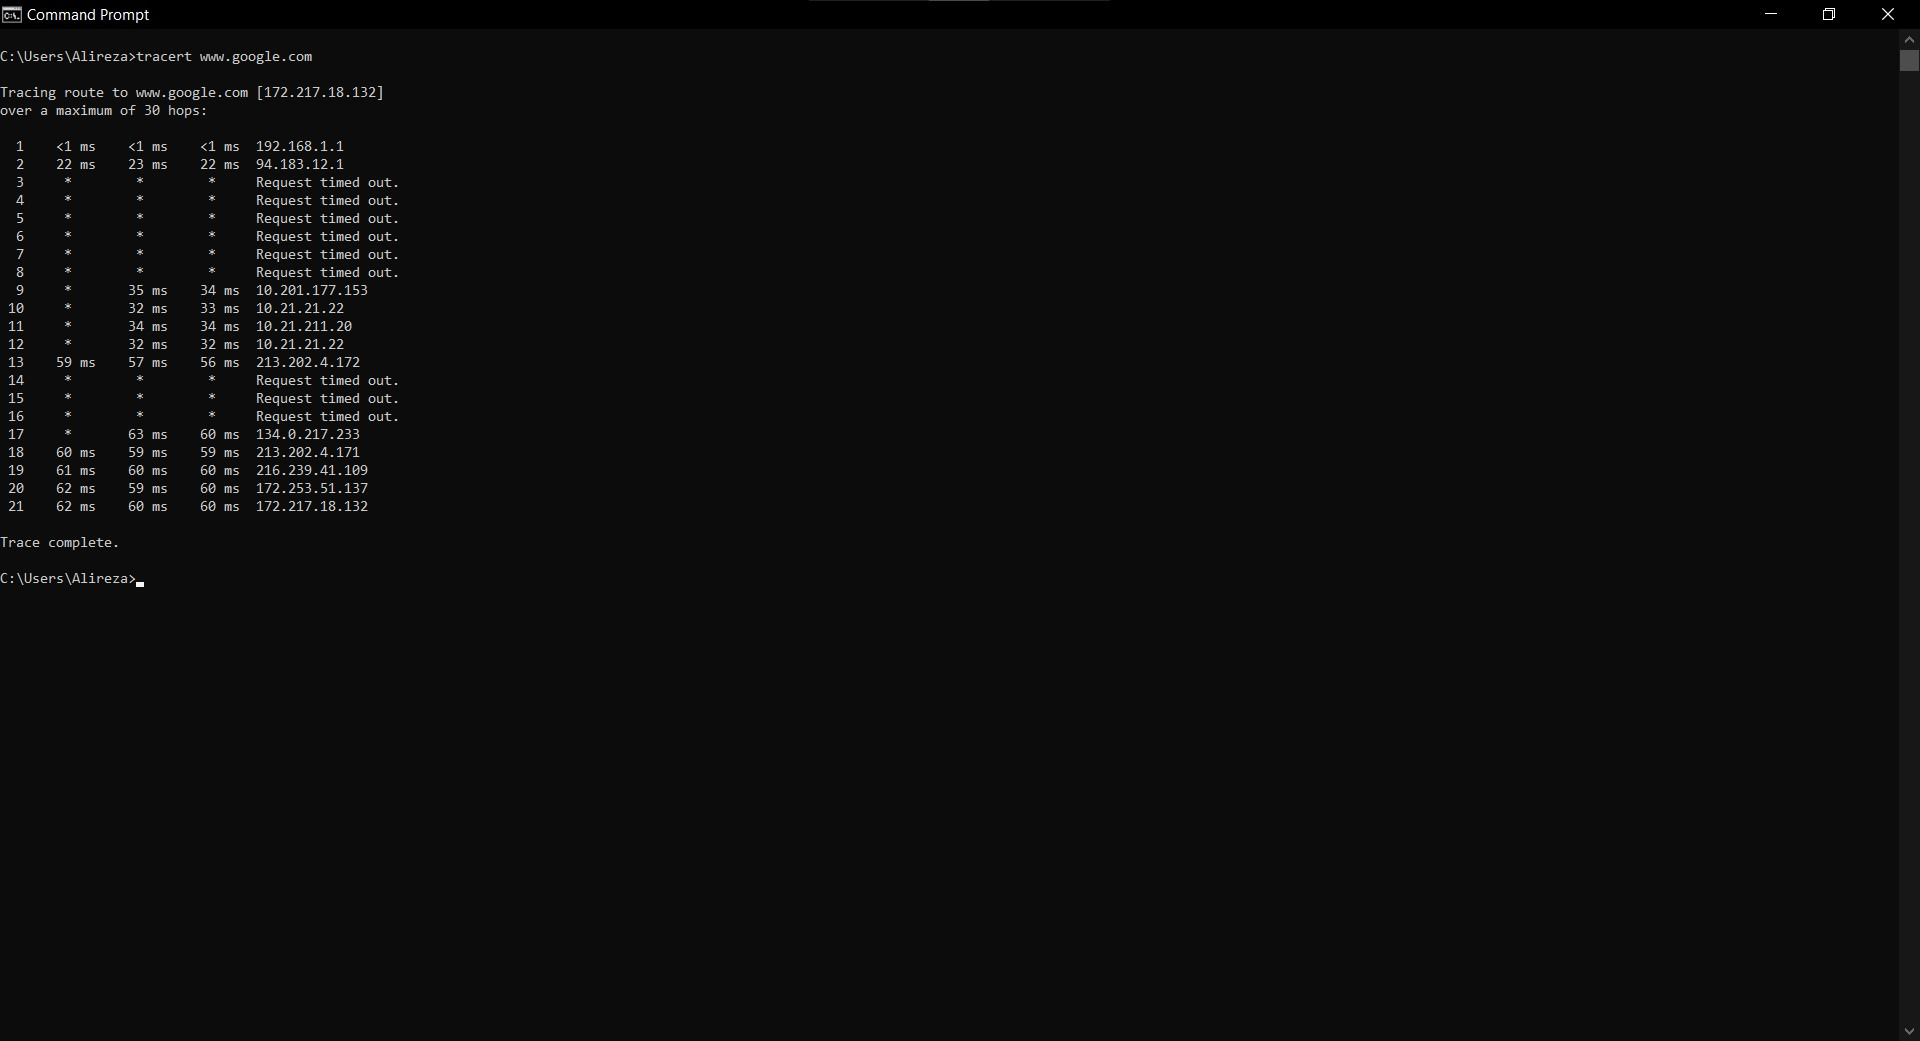
\includegraphics[width=1.0\textwidth]{figures/5.1.jpg}
    \caption
	{
\lr{tracert www.google.com}
	}
    \label{fig:fig1}
\end{figure}

\section{گام ششم}
\lr{nslookup} آدرس \lr{IP} نظیر نام یک \lr{target} را برمی‌گرداند.
\begin{figure}[H]
    \centering
    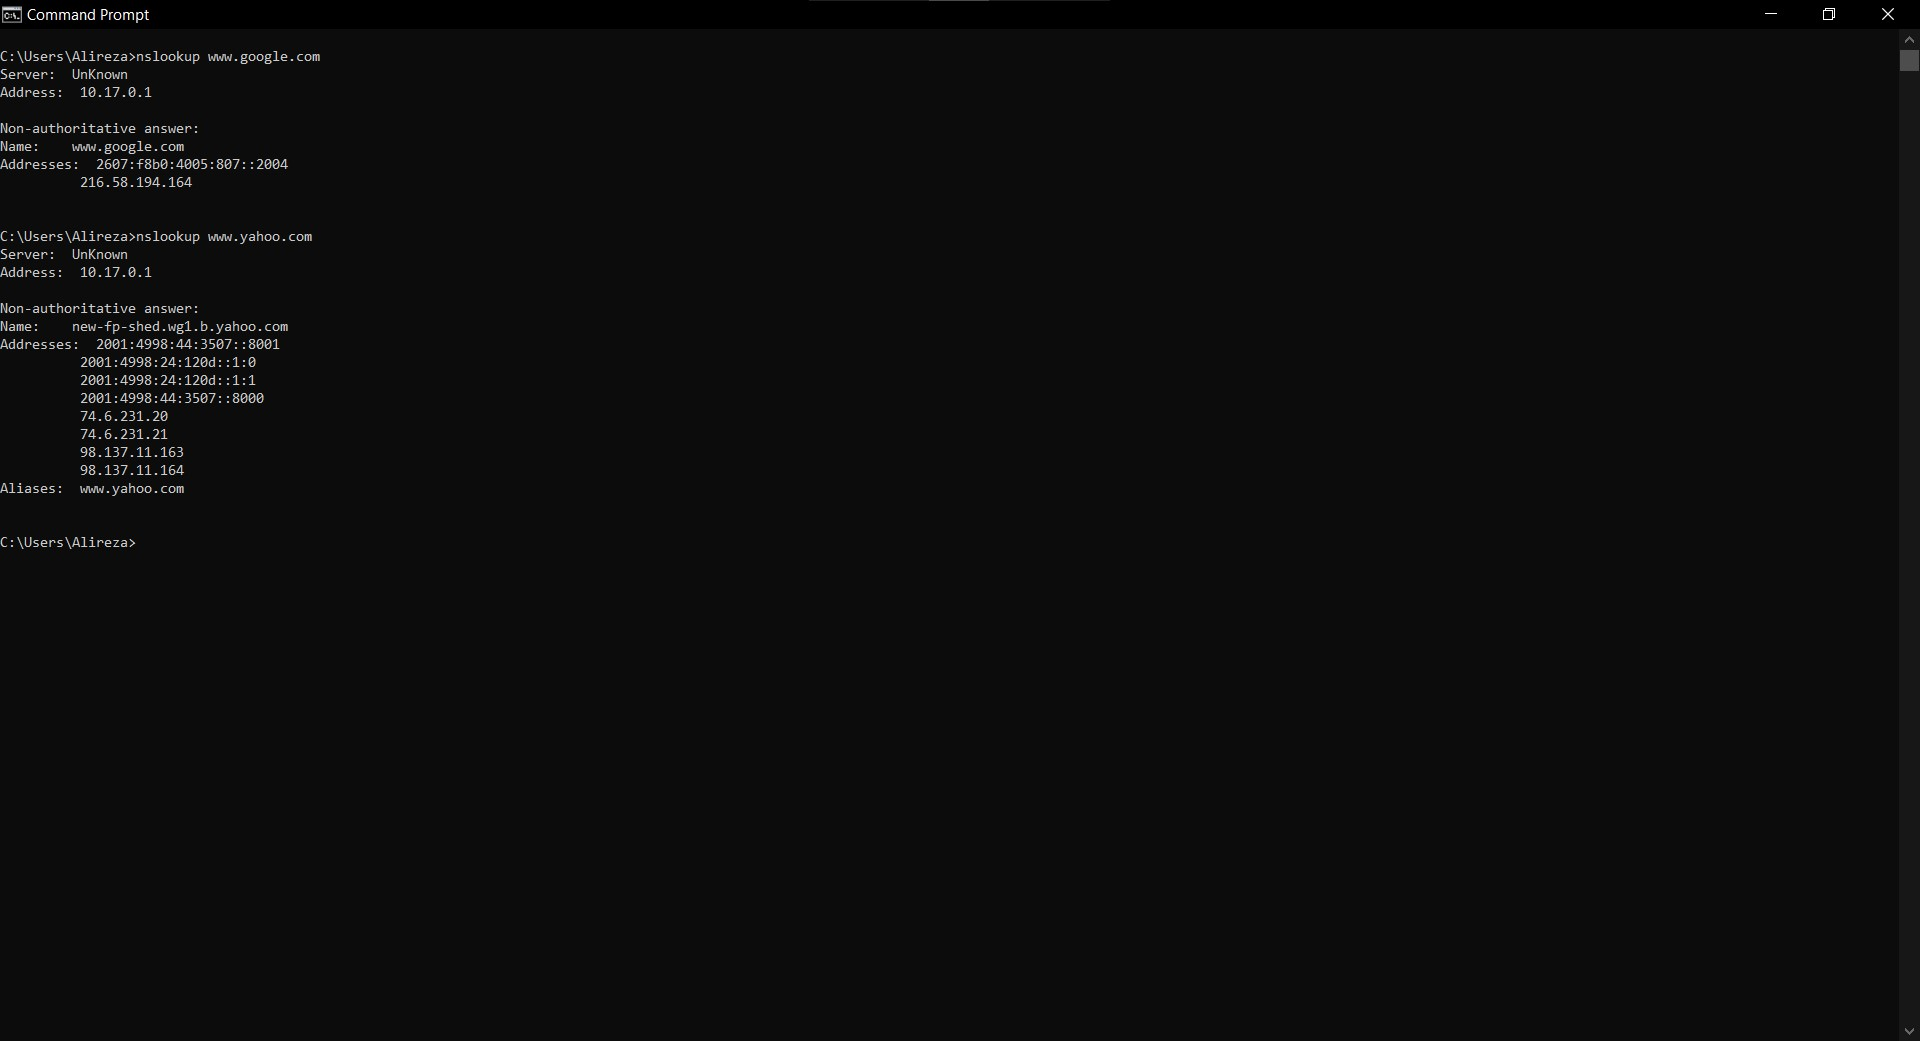
\includegraphics[width=1.0\textwidth]{figures/6.1.jpg}
    \caption
	{
\lr{nslookup www.google.com\\nslookup www.yahoo.com}
	}
    \label{fig:fig1}
\end{figure}

\section{گام هفتم}
\subsection{}
\begin{figure}[H]
    \centering
    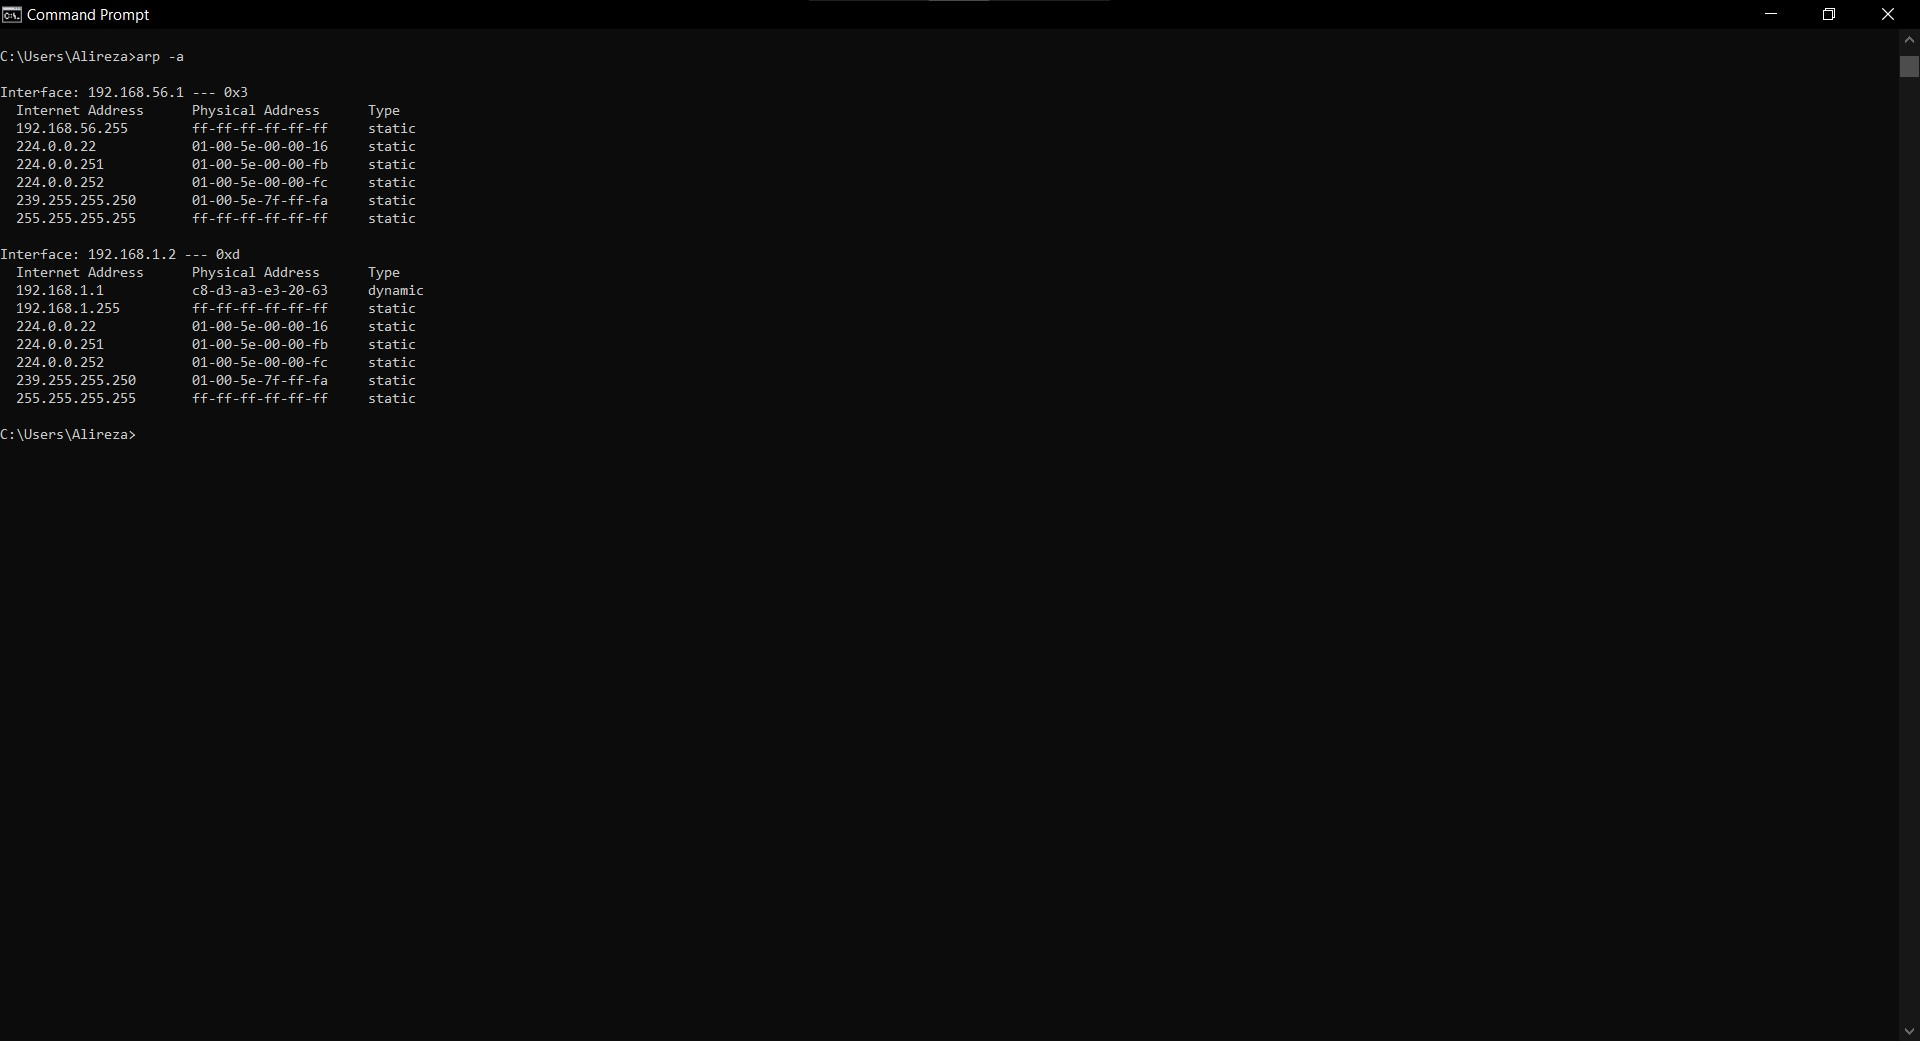
\includegraphics[width=1.0\textwidth]{figures/7.1.jpg}
    \caption
	{
\lr{arp -a}
	}
    \label{fig:fig1}
\end{figure}

\subsection{}
آدرس مورد نظر را به شکل زیر به جدول اضافه می‌کنیم.
\begin{figure}[H]
    \centering
    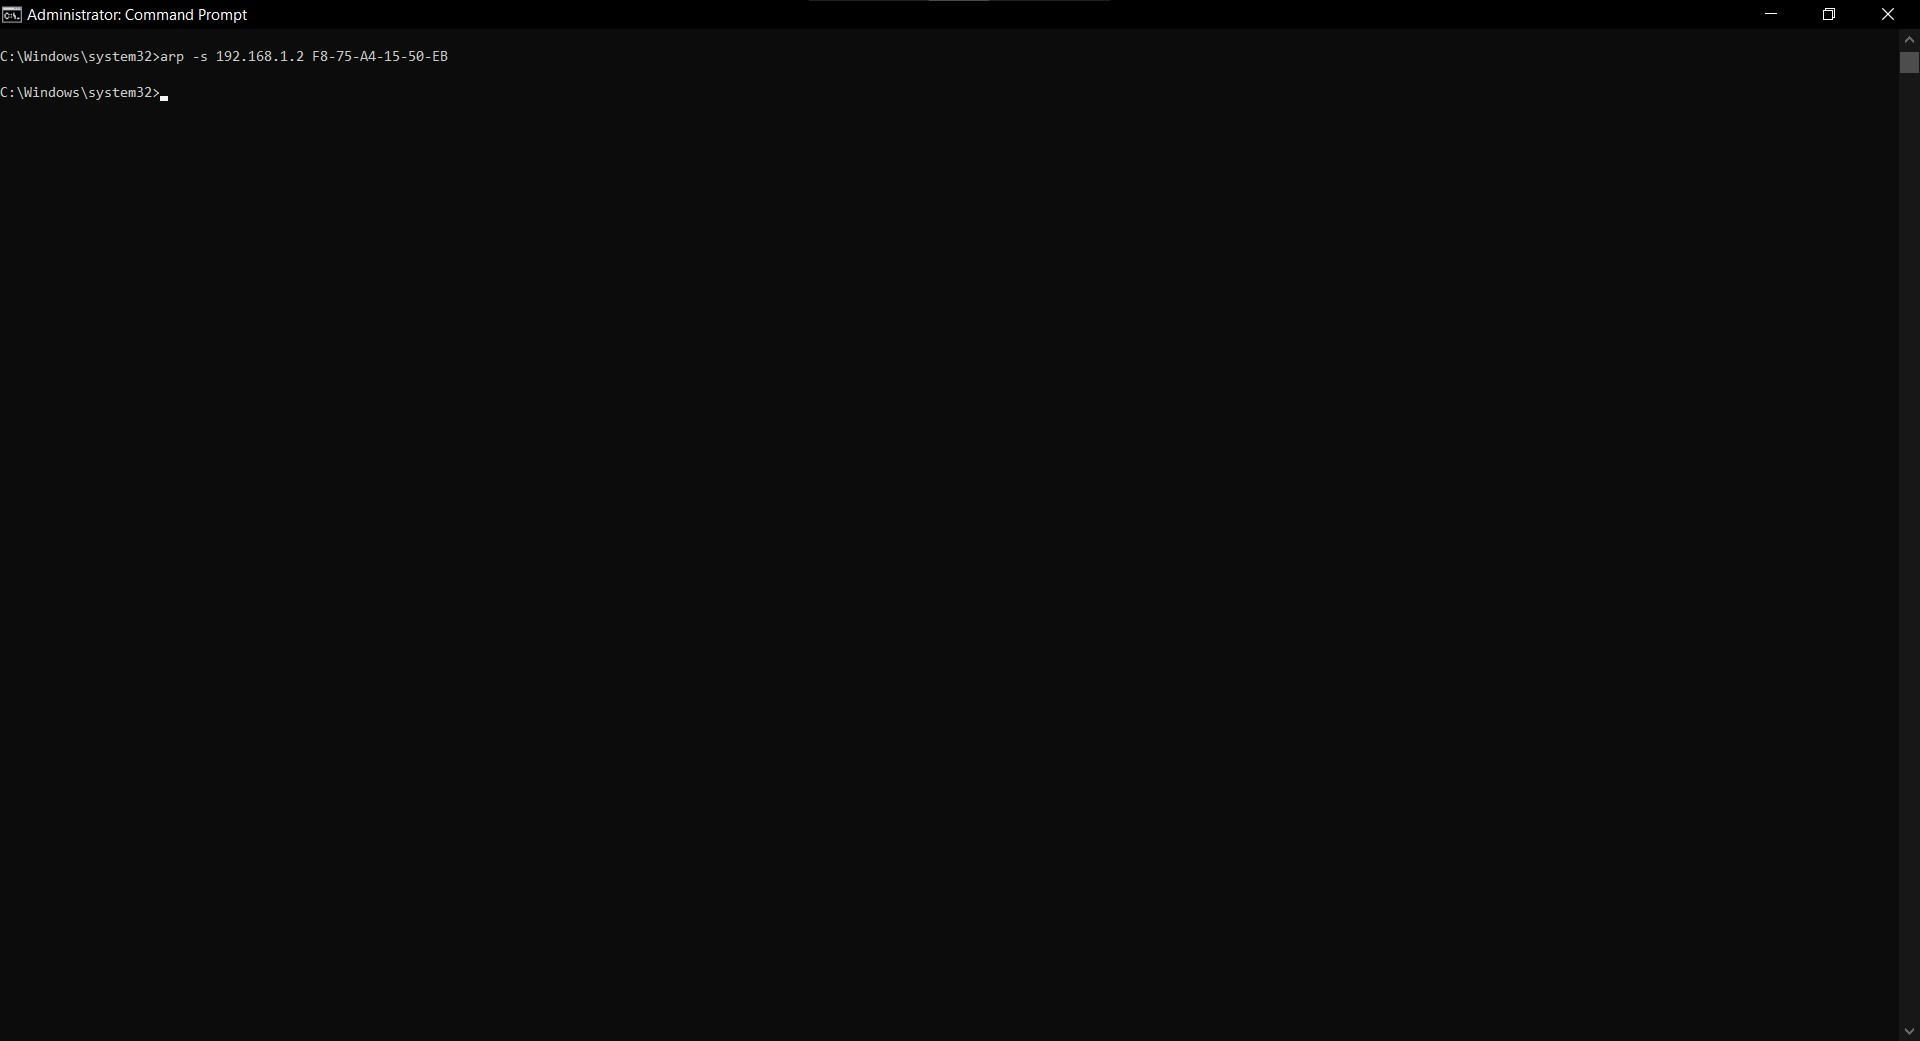
\includegraphics[width=1.0\textwidth]{figures/7.2.jpg}
    \caption
	{
\lr{arp -s 192.168.1.2 F8-75-A4-15-50-EB}
	}
    \label{fig:fig1}
\end{figure}

\subsection{}
\begin{figure}[H]
    \centering
    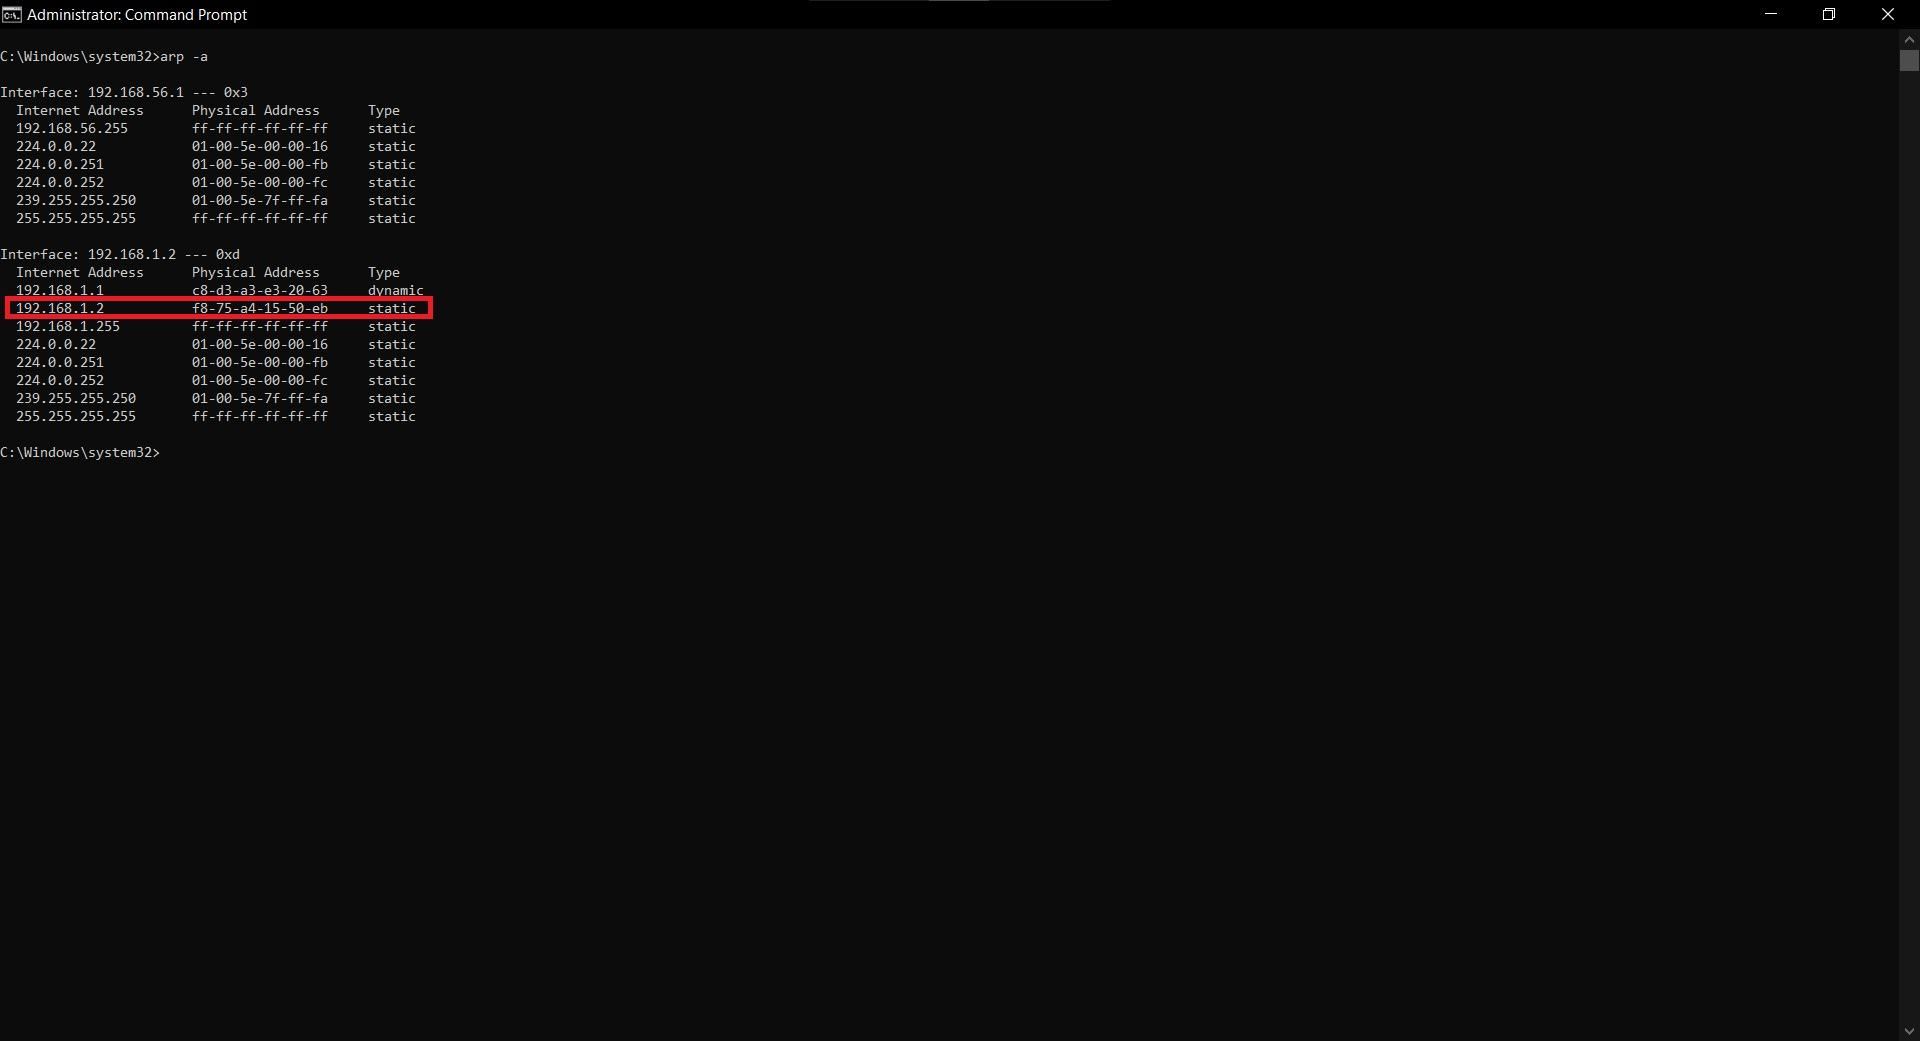
\includegraphics[width=1.0\textwidth]{figures/7.3.jpg}
    \caption
	{
\lr{arp -a}
	}
    \label{fig:fig1}
\end{figure}

\subsection{}
آدرس مورد نظر را به شکل زیر از جدول حذف می‌کنیم.
\begin{figure}[H]
    \centering
    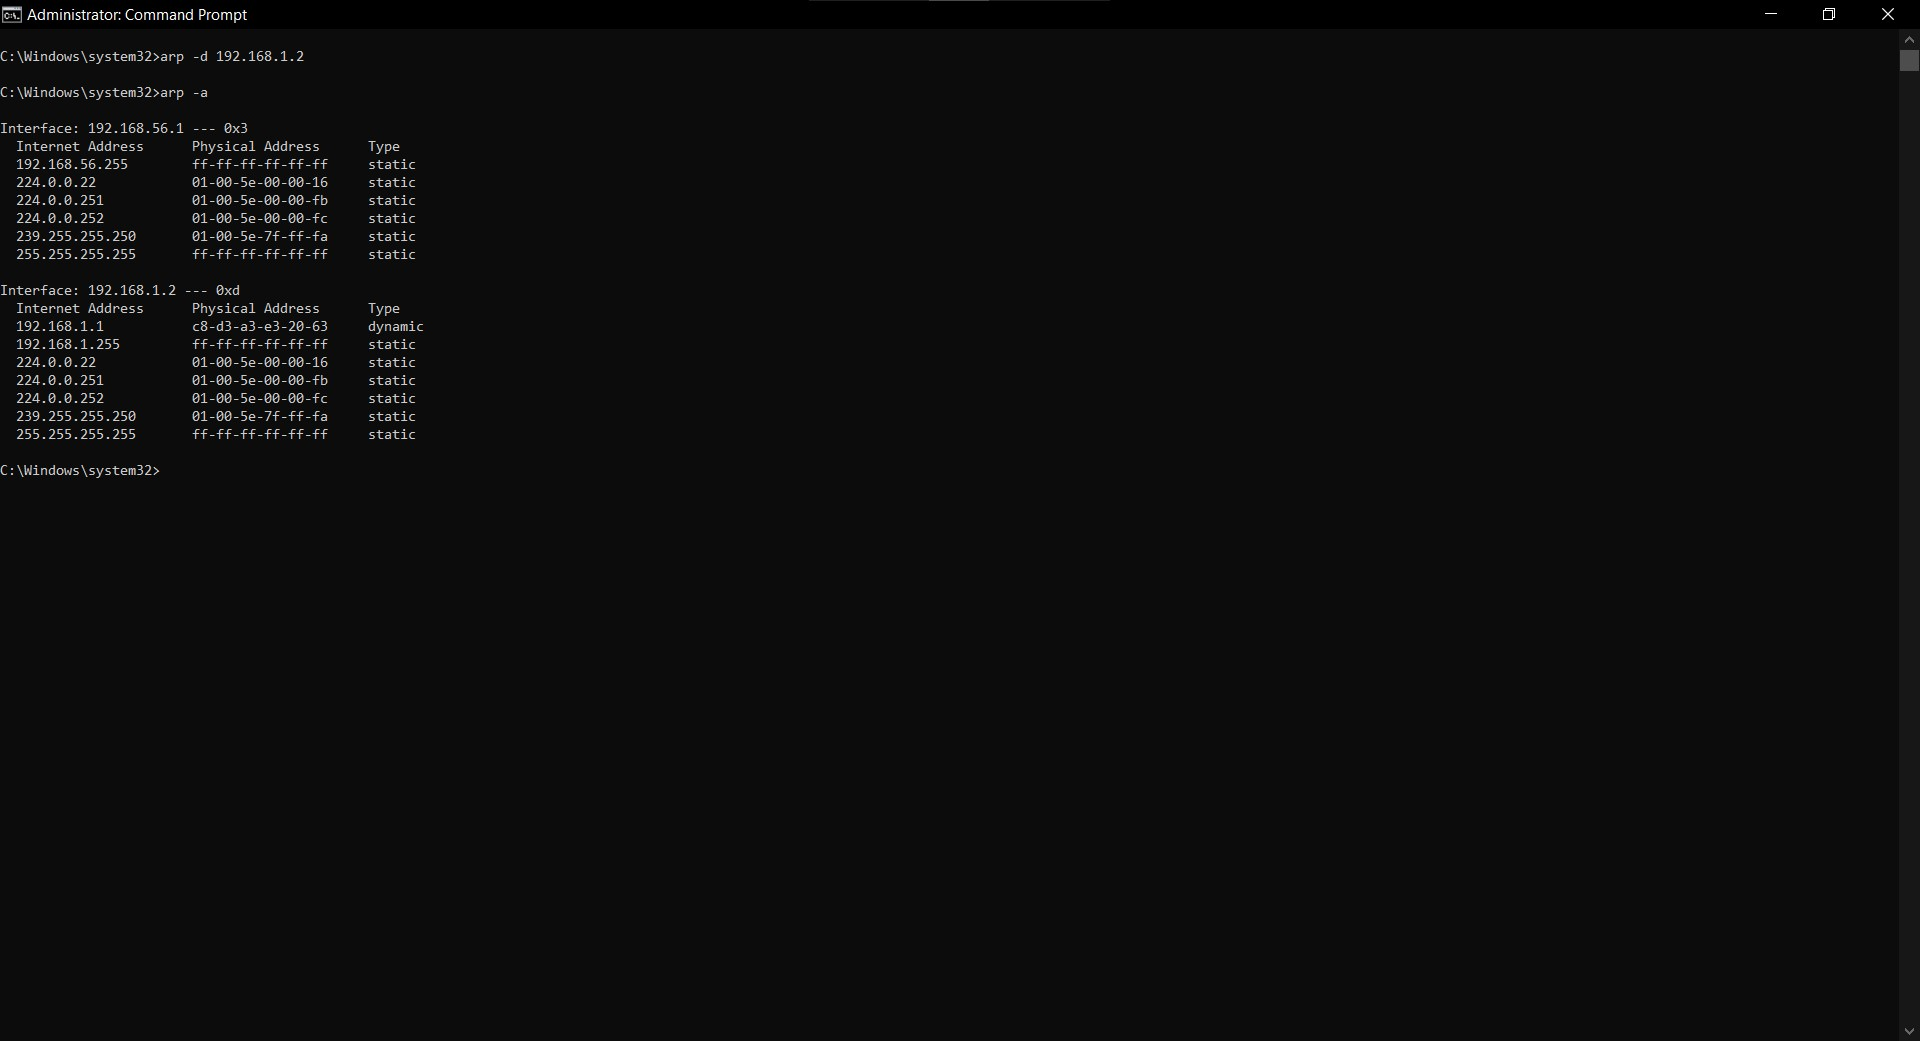
\includegraphics[width=1.0\textwidth]{figures/7.4.jpg}
    \caption
	{
\lr{arp -d 192.168.1.2}
	}
    \label{fig:fig1}
\end{figure}

\section{گام هشتم}
\subsection{}
آپشن \lr{-n} آدرس‌ها و پورت‌ها را به شکل عددی نمایش می‌دهد.
\begin{figure}[H]
    \centering
    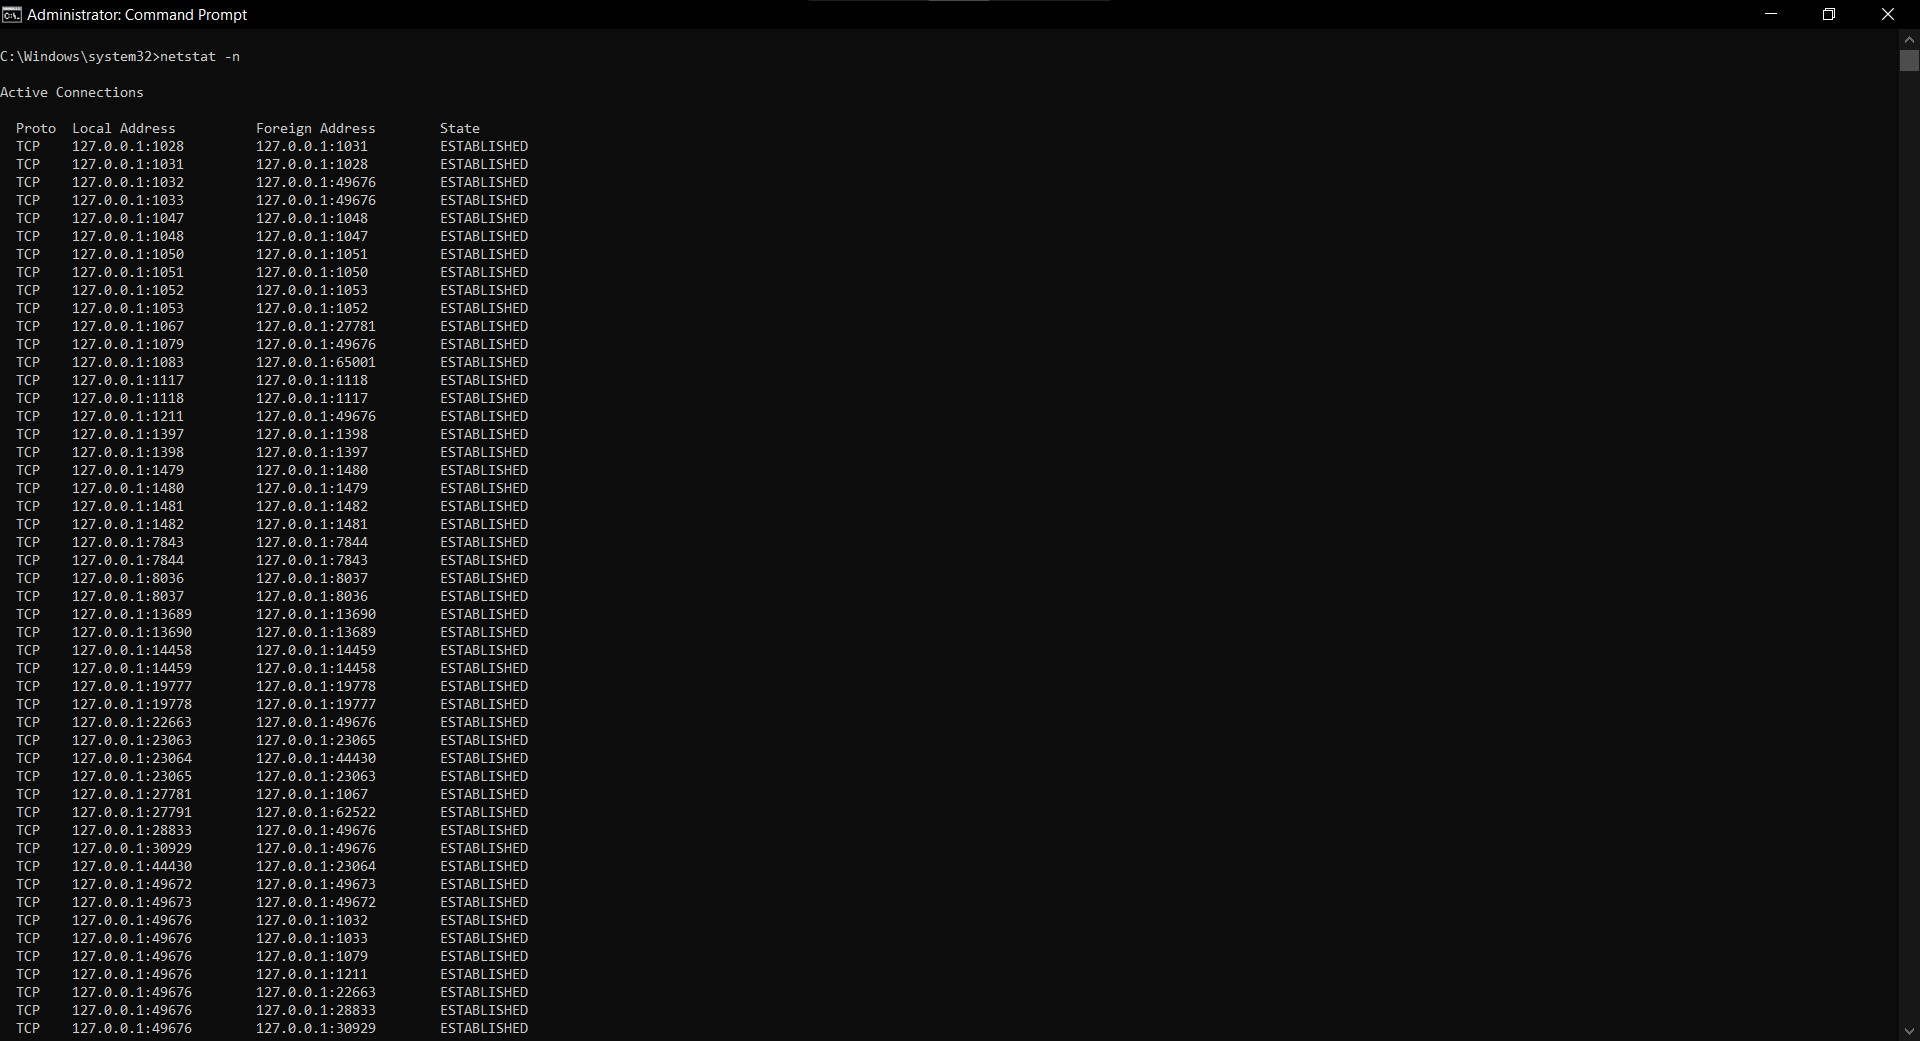
\includegraphics[width=1.0\textwidth]{figures/8.1.jpg}
    \caption
	{
\lr{netstat -n}
	}
    \label{fig:fig1}
\end{figure}
دستور \lr{netstat -a -n} تمامی آدرس‌ها و پورت‌ها را به شکل عددی نمایش می‌دهد.
\subsection{}
\begin{figure}[H]
    \centering
    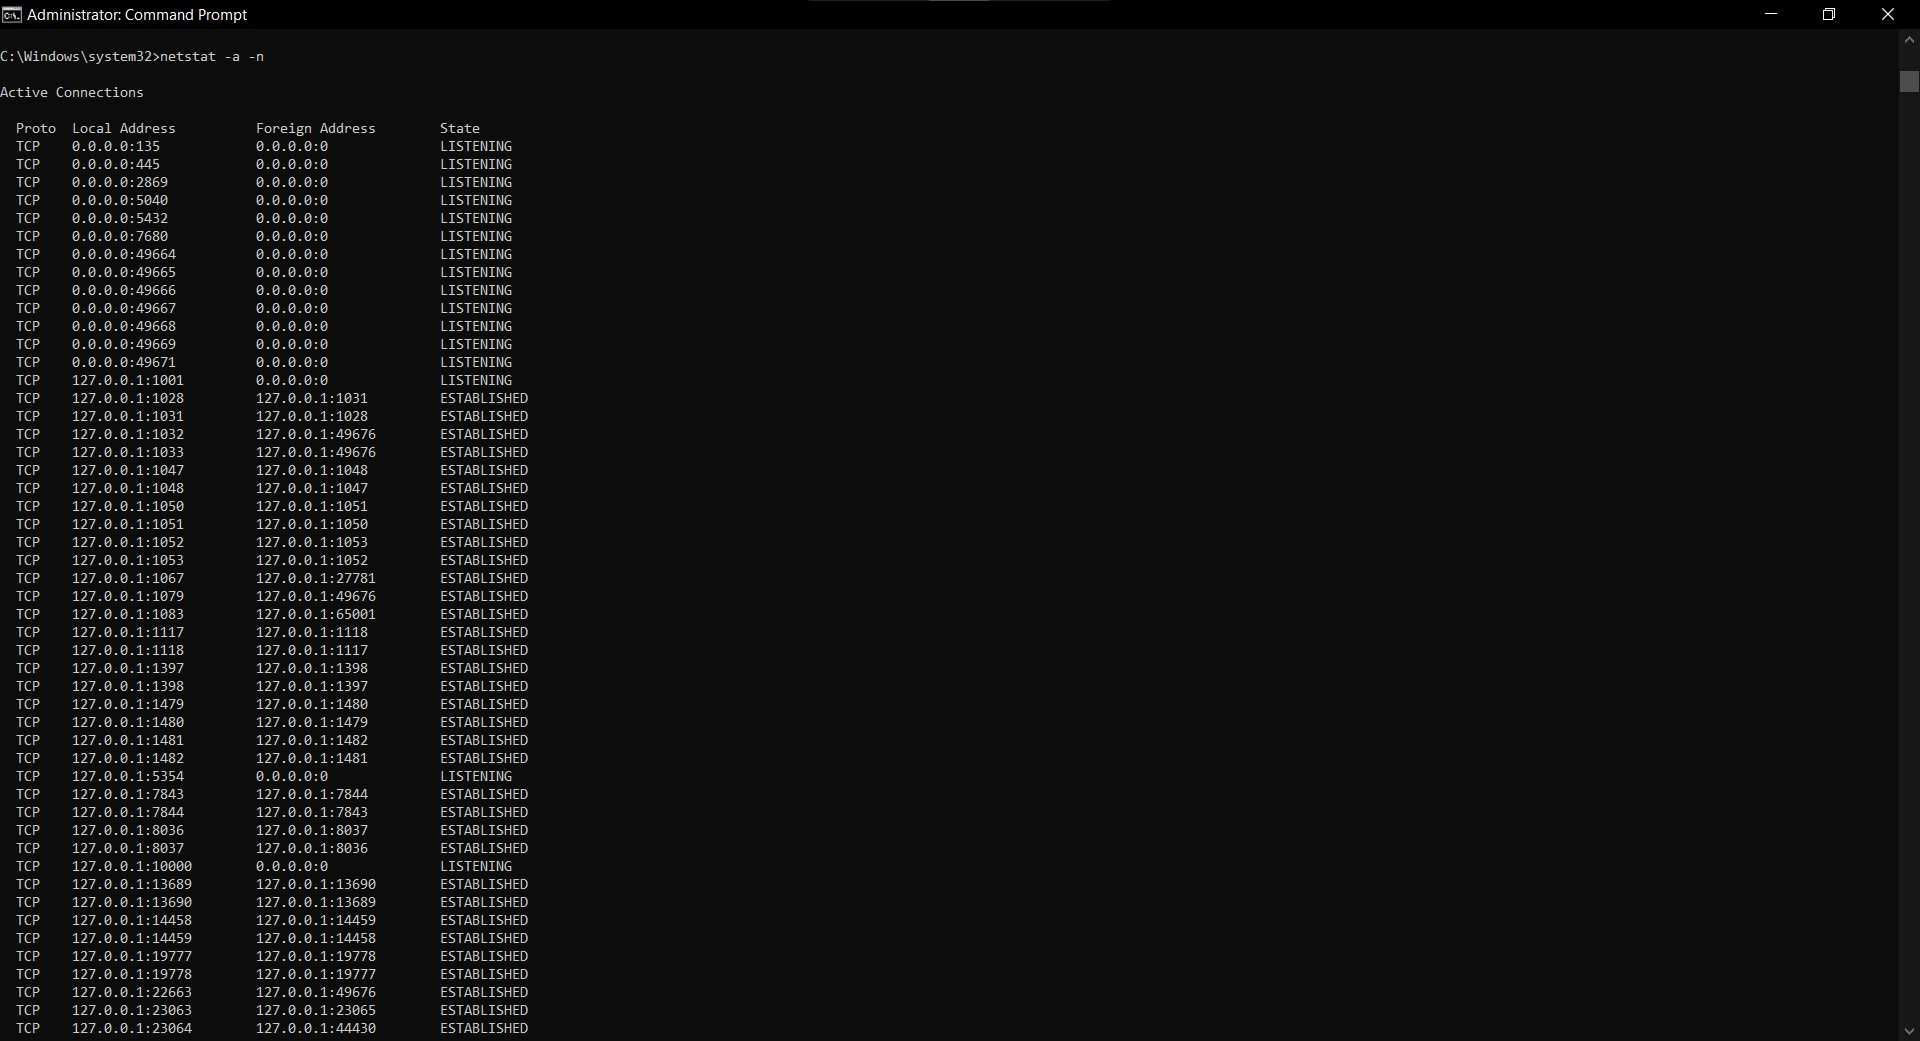
\includegraphics[width=1.0\textwidth]{figures/8.2.jpg}
    \caption
	{
\lr{netstat -a -n}
	}
    \label{fig:fig1}
\end{figure}

\subsection{}
همانطور که در تصویر مشخص است، پروتکل‌های \lr{TCP, UDP, TCPv6, or UDPv6} پشتیبانی می‌شوند و درصورتی که با آپشن \lr{-s} اجرا شود از پروتکل‌های \lr{IP, IPv6, ICMP, ICMPv6, TCP, TCPv6, UDP, or UDPv6} پشتیبانی می‌کند.
\begin{figure}[H]
    \centering
    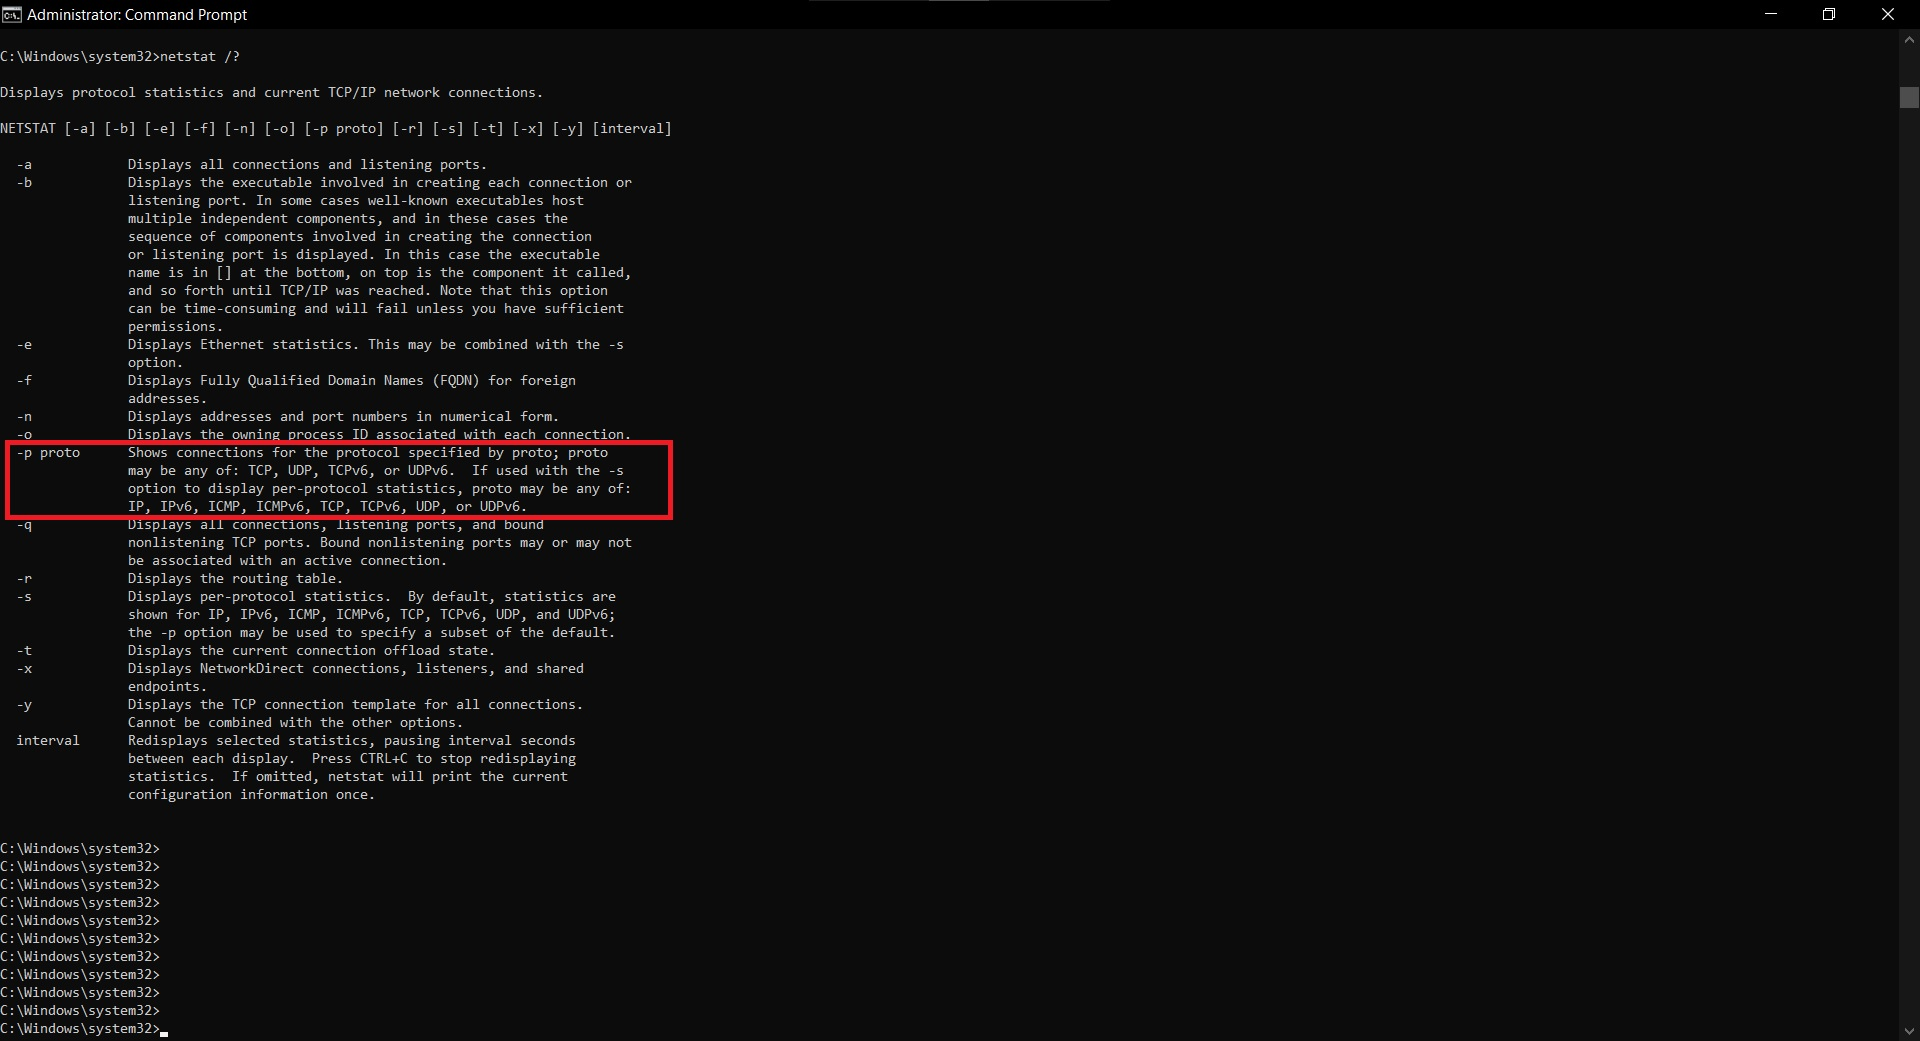
\includegraphics[width=1.0\textwidth]{figures/8.3.jpg}
    \caption
	{
\lr{netstat /?}
	}
    \label{fig:fig1}
\end{figure}

\section{گام نهم}
\subsection{}
\begin{figure}[H]
    \centering
    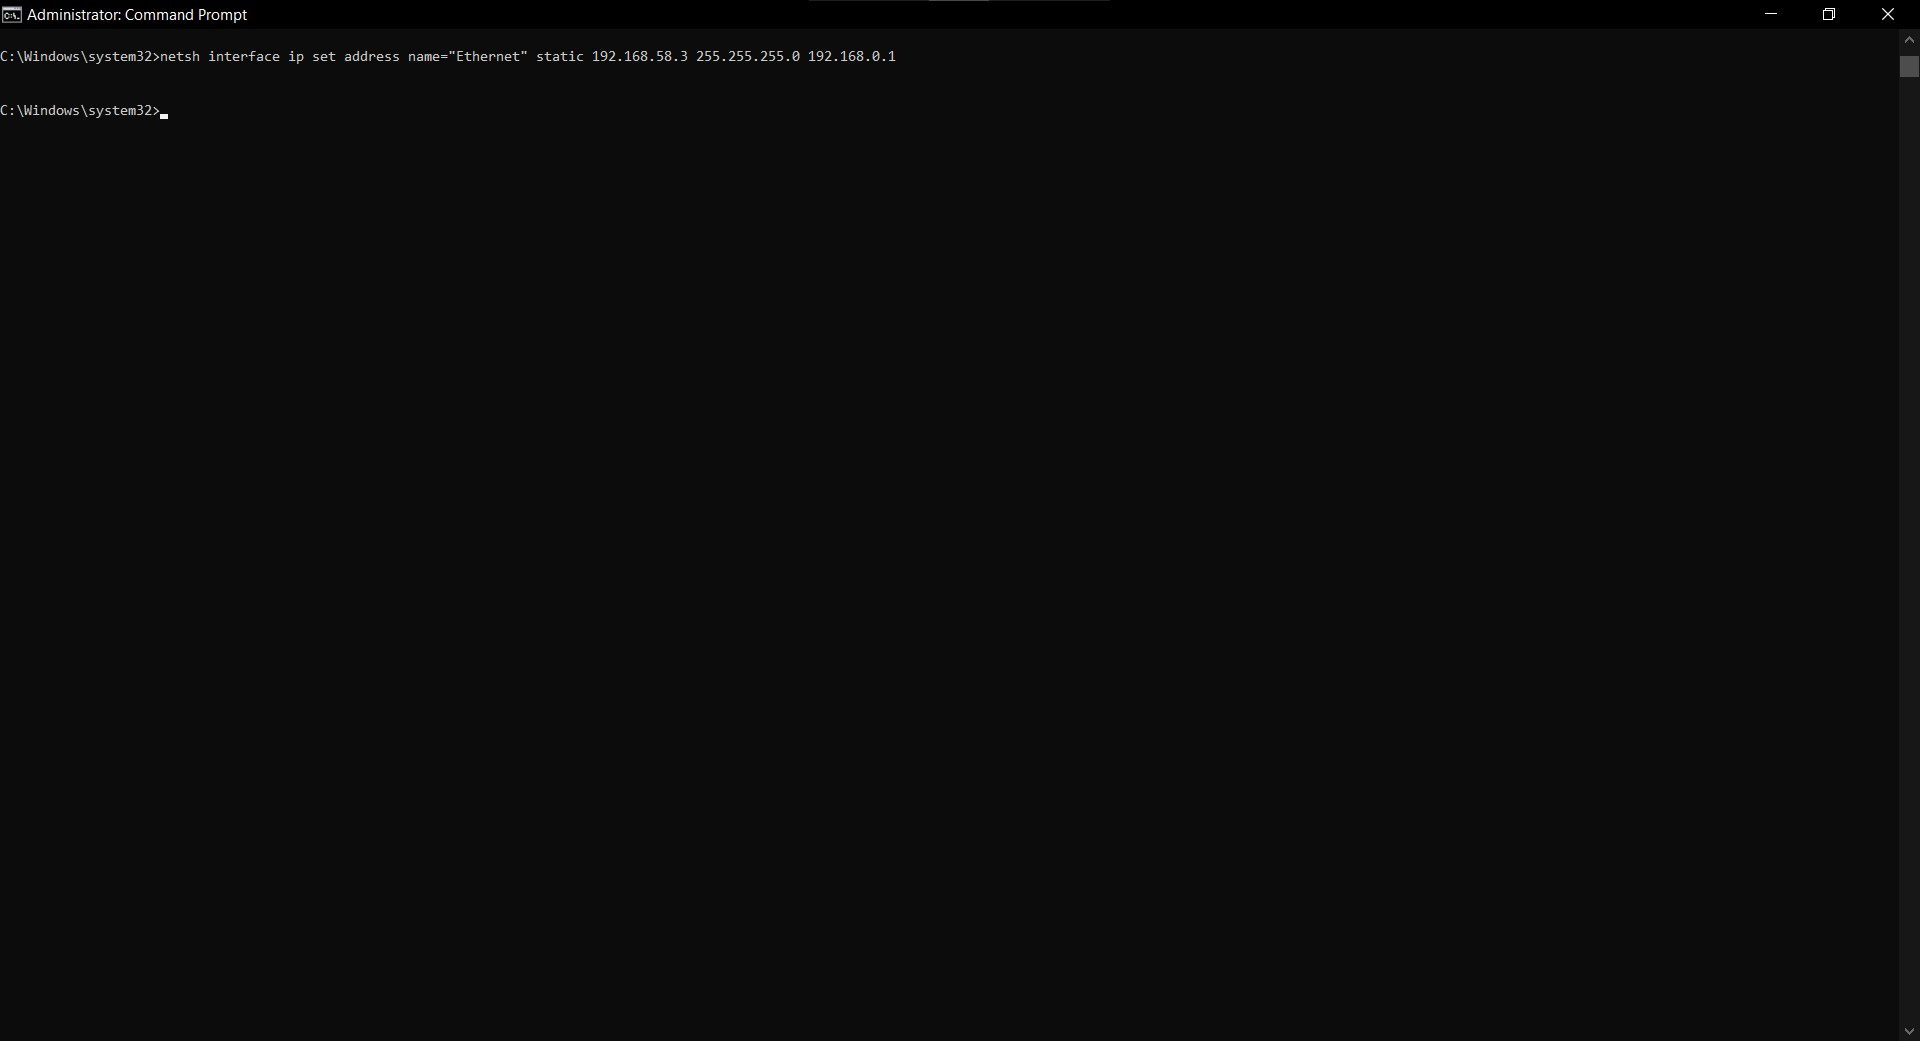
\includegraphics[width=1.0\textwidth]{figures/9.1.jpg}
    \caption
	{
\lr{netsh interface ip set address name="Ethernet" static 192.168.58.3 255.255.255.0 192.168.0.1}
	}
    \label{fig:fig1}
\end{figure}
\subsection{}
\begin{figure}[H]
    \centering
    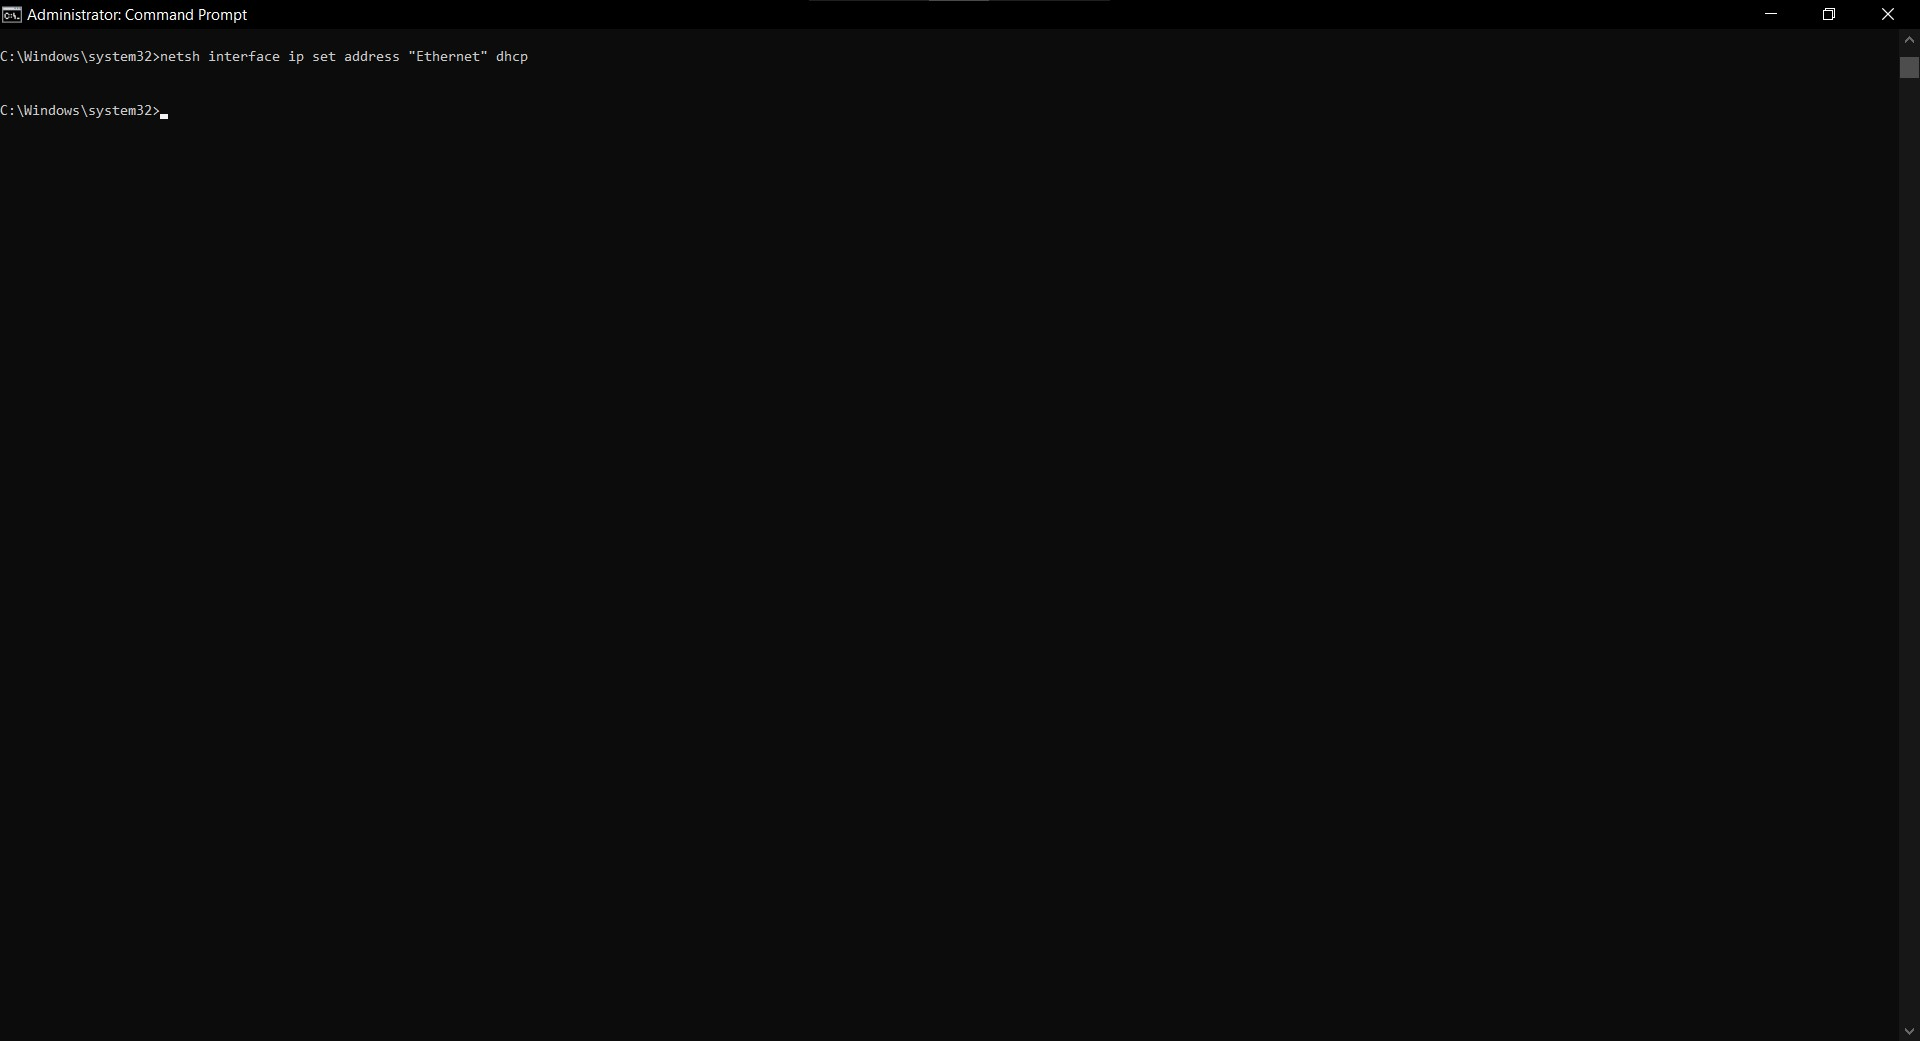
\includegraphics[width=1.0\textwidth]{figures/9.2.jpg}
    \caption
	{
\lr{netsh interface ip set address "Ethernet" dhcp}
	}
    \label{fig:fig1}
\end{figure}
\subsection{}
\begin{figure}[H]
    \centering
    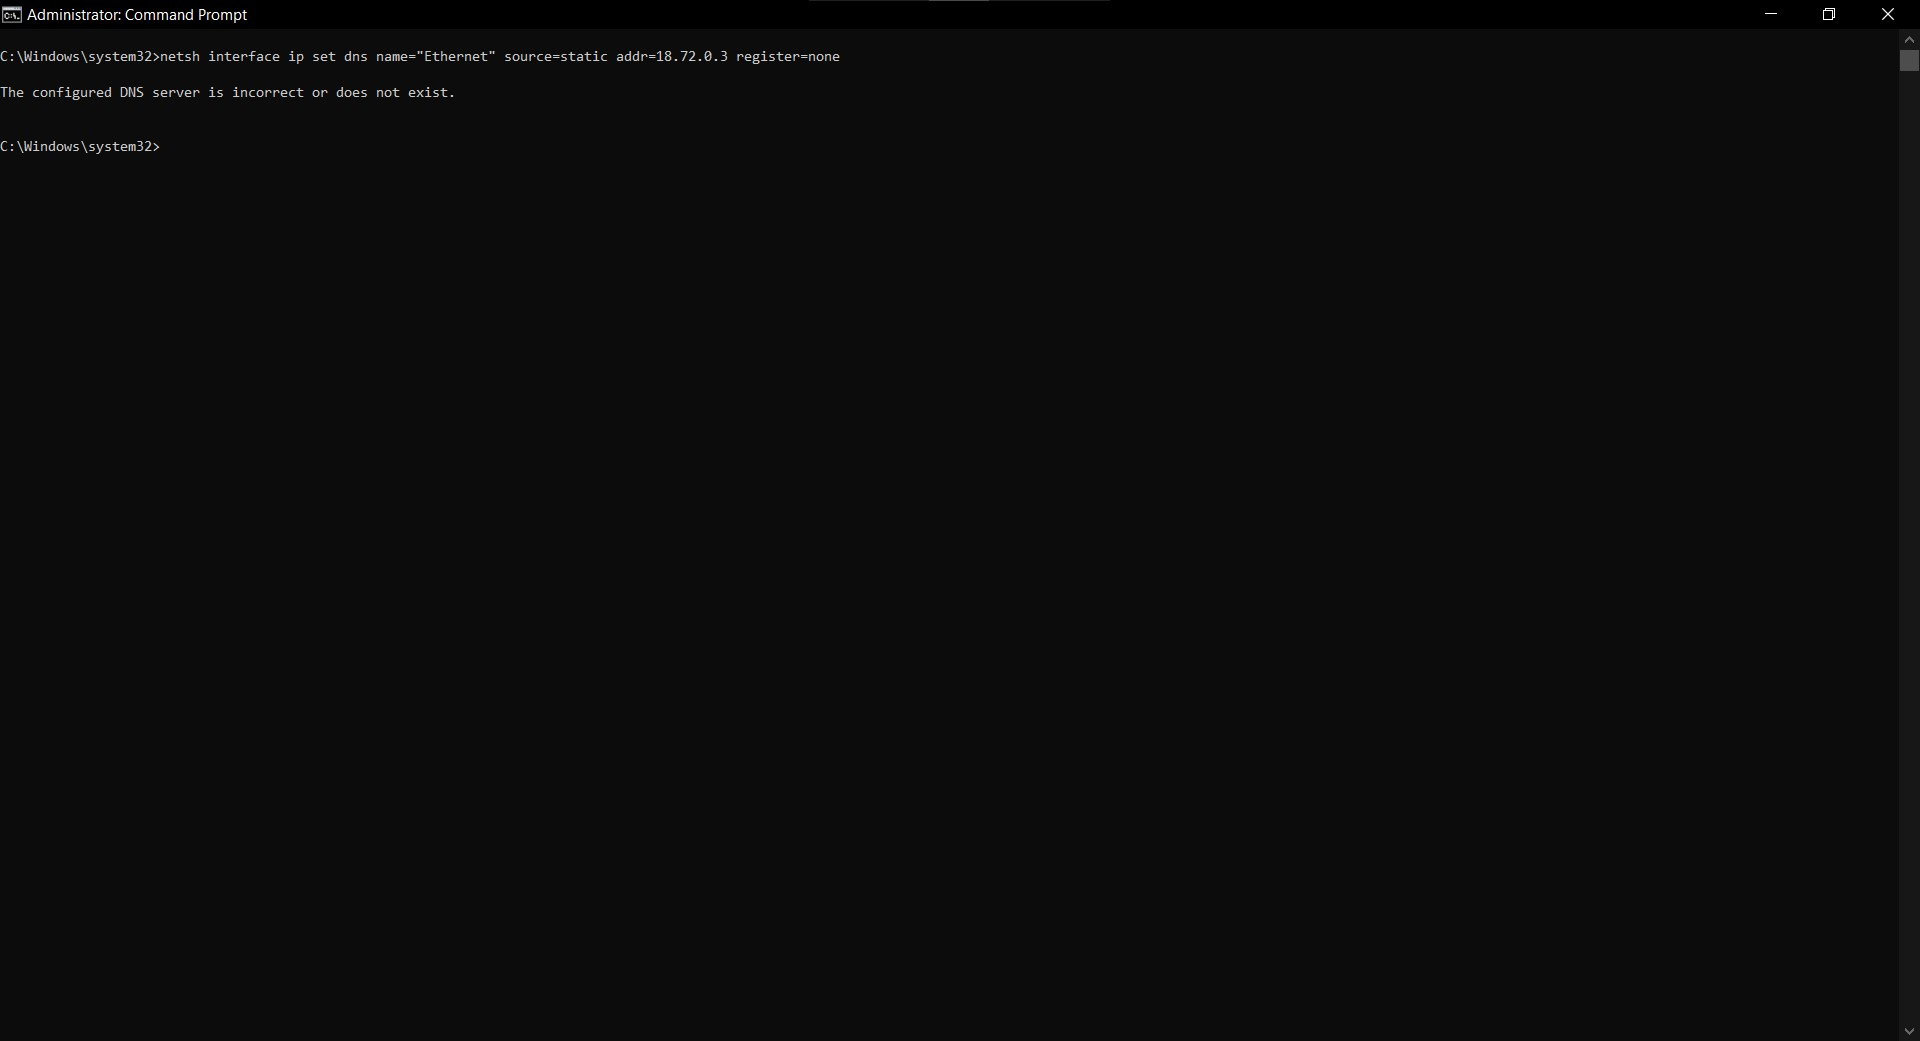
\includegraphics[width=1.0\textwidth]{figures/9.3.jpg}
    \caption
	{
\lr{netsh interface ip set dns name="Ethernet" source=static addr=18.72.0.3 register=none}
	}
    \label{fig:fig1}
\end{figure}
\subsection{}
\begin{figure}[H]
    \centering
    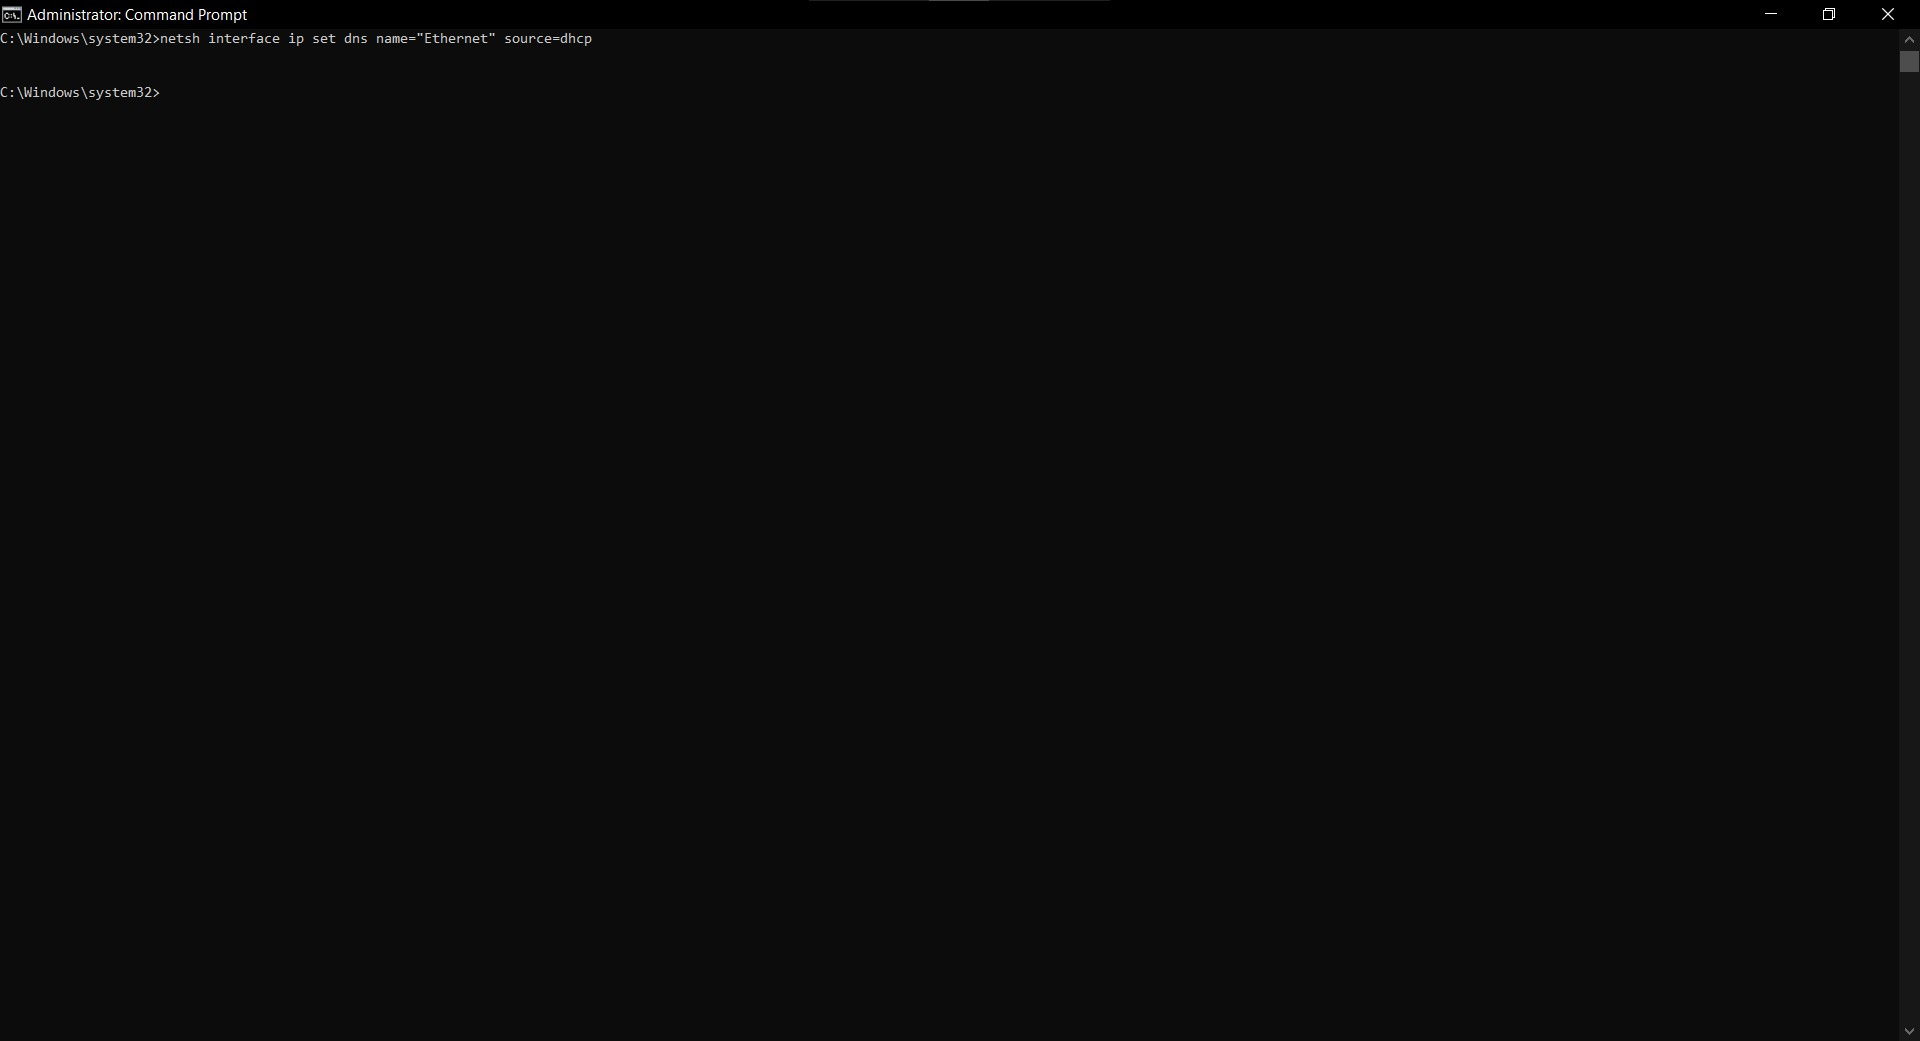
\includegraphics[width=1.0\textwidth]{figures/9.4.jpg}
    \caption
	{
\lr{netsh interface ip set dns name="Ethernet" source=dhcp}
	}
    \label{fig:fig1}
\end{figure}

\section*{منابع}
\renewcommand{\section}[2]{}%
\begin{thebibliography}{99} % assumes less than 100 references
%چنانچه مرجع فارسی نیز داشته باشید باید دستور فوق را فعال کنید و مراجع فارسی خود را بعد از این دستور وارد کنید


\begin{LTRitems}

\resetlatinfont

\bibitem{b1} 
\end{LTRitems}

\end{thebibliography}


\end{document}
